\documentclass{article}

% The LaTeX-to-CNXML translator makes use of Tralics, a LaTeX-to-XML conversion
% utility.  Tralics has implemented all the packages in the LaTeX base directory,
% and it also supports a good number of supplemental LaTeX packages.  These
% supplemental packages are included in the \usepackage{} statements below.
% Packages not in the LaTeX base directory or \usepackage{} statements in this
% template are not supported by Tralics and, hence, not supported by the
% LaTeX-to-CNXML converter.

% If you have a question as to whether a specific LaTeX command is supported,
% please refer to the "HTML Documentation of all TeX commands" section at
% http://www-sop.inria.fr/apics/tralics/.  Here you will find links to manual pages
% organized alphabetically by the first letter of the command.  These pages indicate
% how Tralics handles conversion of each supported command, which informs how the
% LaTeX-to-CNXML translator behaves.

% To prepare your LaTeX document for import, copy the body of that document from its
% source and paste it into this template between the \begin{document} and \end{document}
% statements.  Do not attempt to use any packages other than the ones contained in this
% template.  You may, however, insert user-defined macros directly in this template
% before the \begin{document} statement.  Following this preparation, check to see if
% your template-compliant document can generate a .dvi (.pdf) using latex (pdflatex).
% If so, then your document is ready for import; if not, you must modify your document
% to generate an output file using only the packages supported by Tralics as described
% above.

% Tralics supports the following AMS packages
% (see http://www-sop.inria.fr/apics/tralics/packages.html for details on full/partial
% support of package commands)
\usepackage{amsbsy,amscd,amsfonts,amsgen,amsmath,amsopn,amssymb,amstext,amsthm,amsxtra}

% Tralics supports \includegraphics and \scalebox, but not all other graphicx package
% commands; check the web documentation on supported commands before attempting to use
% other commands in the graphicx package:
\usepackage{graphicx}

% We must specifically invoke the verbatim package as follows to direct Tralics to handle
% the verbatim environment properly:
\usepackage{verbatim}

% Tralics also allows the following packages:
% (see http://www-sop.inria.fr/apics/tralics/packages.html for details on full/partial
% support of package commands)

%\usepackage{alltt}
%\usepackage{array}
%\usepackage{bracket}
%\usepackage{calc}
%\usepackage{delarray}
%\usepackage{eucal}
%\usepackage{eufrak}
\usepackage{fancyvrb}
%\usepackage{fix-cm}
%\usepackage{fixltx2e}
%\usepackage{flafter}
%\usepackage{fontenc}
%\usepackage{fp}
%\usepackage{graphpap}
%\usepackage{html}
%\usepackage{ifthen}
%\usepackage{index}
%\usepackage{inputenc}
%\usepackage{latexsym}
%\usepackage{lipsum}
%\usepackage{makeidx}
%\usepackage{minimal}
%\usepackage{mml}
%\usepackage{natbib}
%\usepackage{newlfont}
%\usepackage{oldlfont}
%\usepackage{shortvrb}
%\usepackage{showidx}
%\usepackage{soul}
%\usepackage{syntonly}
%\usepackage{textcase}
%\usepackage{textcomp}
%\usepackage{tloop}
%\usepackage{theorem}
%\usepackage{upref}

%-------------------------------------------------------------------
% You can insert user-defined macros (using the supported packages
% only) here...

%-------------------------------------------------------------------


%-------------------------------------------------------------------
% Begin entering your LaTeX document content here...
\begin{document}

%Throughout this module, we will use the programming language MATLAB (or Octave).  For an introduction to MATLAB, see here (``Introduction to MATLAB and scripts"  http://cnx.org/content/m13554/latest/ ).


%\section{Neuroscience Motivation}
%
%\subsection{Epilepsy}
%
%\subsection{Neural Activity}
%The basic unit of the brain is a cell called a neuron.  Neurons consist of a central cell body with outreaching arms that connect to other neurons.  An adult brain has about 100 billion neurons, and each neuron can have up to 10,000 connections.  Neurons transmit information by chemical releases and electrical impulses.  The electrical action of brain activity affects the potential of the surrounding brain matter.  When billions of neurons act in concert, these electronic potentials collect, and patterns of activity can be seen in the overall voltage of the group of neurons.
%
%\subsection{EEG}
%Brain waves can be measure by a method called {\it electroencephalography} (EEG).  The measuring equipment consists of tens of electrode sensors placed on the head (fig. 1) that record electric pulses.  Each sensors outputs a series of data points that represent a "brain wave." (figure 2)

\section*{Brain Waves and the EEG}
Signals are sent through the brain using both chemical and electrical means.  The synchronized electrical activity of individual neurons adds up to something big enough to detect on from outside the head.  To measure it, we use a set of electrical nodes called an electroencephalogam (EEG).  The measured activity reflects different states of the brain which in turn tell us something about the mindset of the person.  Our goal in this module is to decompose an EEG signal into its different frequencies, which is intuitively the most meaningful piece of information.

\section{All About Waves}
Brainwaves have complex shapes that are not easily interpreted.  In order to study these waves, we need to develop some mathematical tools that will tell us about different waves.  To outline, we begin by talking about pure (sine or cosine) waves, then move to the trapezoid rule for estimating area under a curve.  Next, we develop Fourier analysis for picking out the frequencies in a jumbled signal, and finally use these tools to create spectrograms, which allow us to track different frequencies over time.


\subsection{Sine Waves}
The sine wave is a mathematical function.  It describes many physical phenomena, including sound waves and oscillation.  It looks just like a wave.  MATLAB uses the {\tt sin} function to make sin waves.  For example, to make Figure 1, we use the code: 

\begin{verbatim}
t = 0:.01:1;
y = sin(2*pi*t);
plot(t,y);
\end{verbatim}

The sine wave is defined by the lengths and angles of a triangle.  Run {\tt sincirc.m} (copied below) to see how the sine and cosine values relate to the angle $\varphi$ of the triangle.  As you can see, if $\varphi$ is the angle of a right triangle with hypotenuse $1$ (illustrated by the circle) , $\sin(\varphi)$ is the height of the triangle and $\cos(\varphi)$ is the base of it:

%\begin{figure}[htbp]
%\begin{center}
%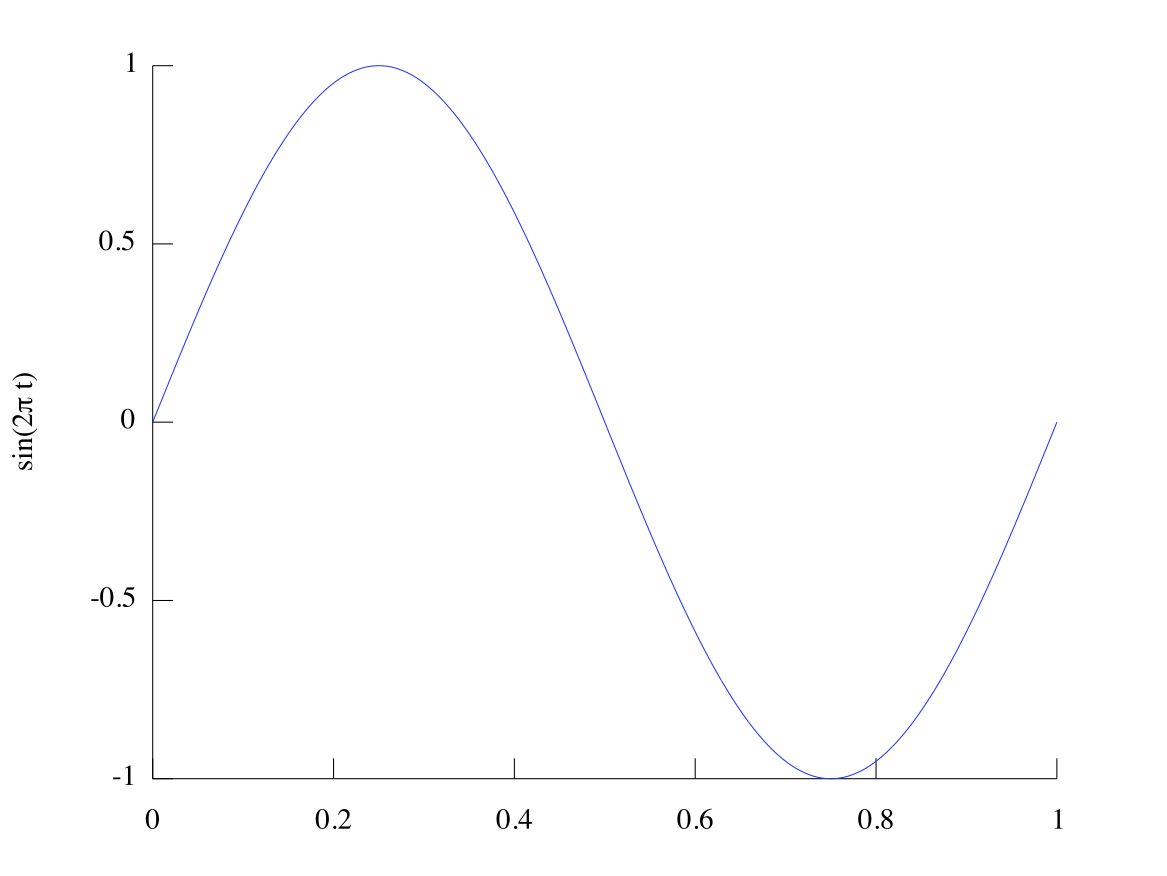
\includegraphics[scale=0.4]{simple_sin.pdf}
%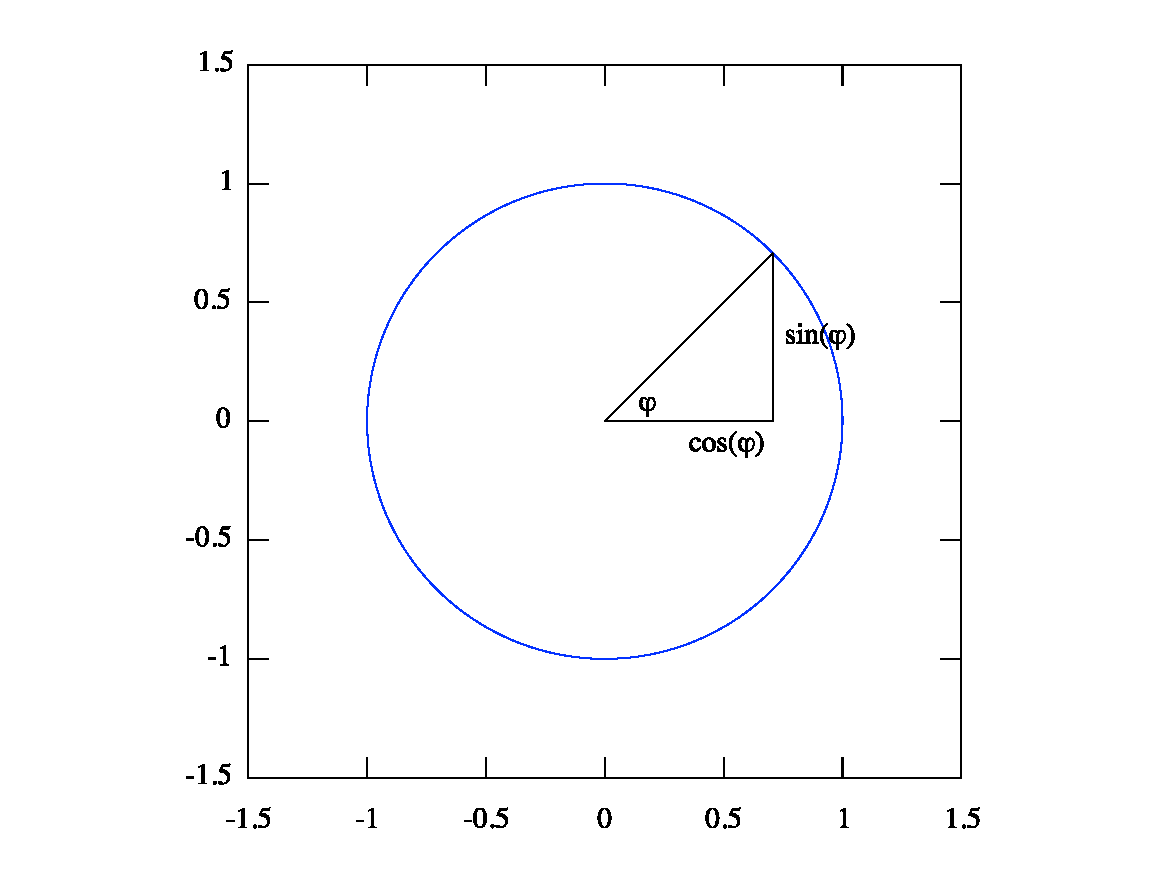
\includegraphics[scale=0.4]{circsinpic.pdf}
%\caption{Left: A sine wave.      Right: the relation of sine and cosine to the triangle.}
%\label{default}
%\end{center}
%\end{figure}



%unused
%\begin{figure}[htbp]
%\begin{center}
%  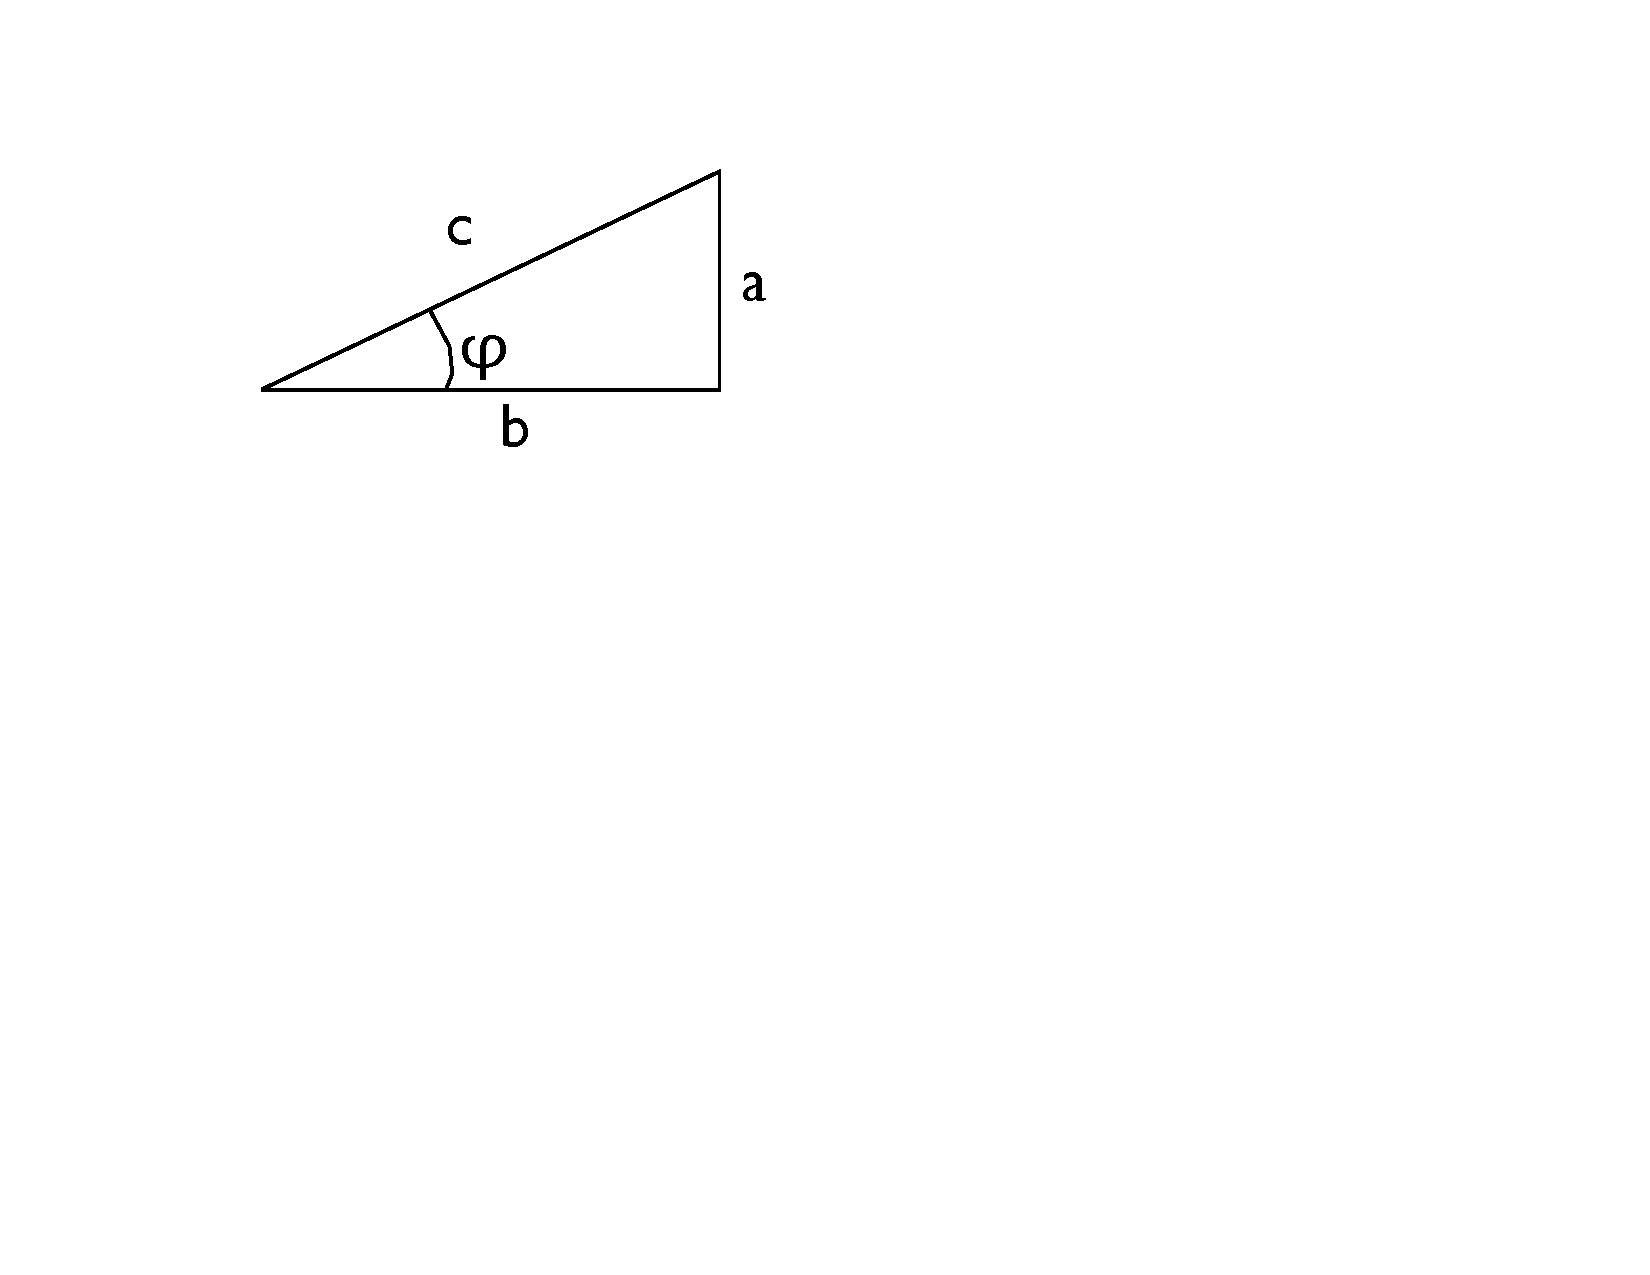
\includegraphics[scale=0.7]{final_tri.pdf}
%\caption{Relations of the sin wave within a triangle}
%\label{default}
%\end{center}
%\end{figure}


%\[\sin(\varphi) = \frac{a}{c}\]
%Likewise, the $cosine$ function describes a different relation within the triangle:
%\[\cos(\varphi) = \frac{b}{c}\]







\begin{verbatim}
% sincirc.m
%
% sincirc.m illustrates the relation of the sin and cosine waves to the circle.

%define parameters
Nturns = 2;
steps_per_turn = 9;
step_inc = 2*pi/steps_per_turn;

%set up points for circle
circ_x = cos(0:.01:2*pi);
circ_y = sin(0:.01:2*pi);
axis equal

%loop over triangles with different angles
for n = 1:Nturns * steps_per_turn;
    phi = n * step_inc + pi/4;

    %plot circle, then triangle, then text
    plot(circ_x, circ_y);
    axis([-1 1 -1 1] * 1.5);
    line([0 cos(phi)], [0 sin(phi)]);
    line([1 1] * cos(phi), [0 sin(phi)]);
    line([0 cos(phi)], [0 0]);
    text(cos(phi)/2 , -.1*sign(sin(phi)),'cos(\varphi)')
    text(cos(phi) + .1*(sign(cos(phi))-.5), sin(phi)/2, 'sin(\varphi)')
    text(cos(phi)*.2, sin(phi)*.1,'\varphi');
    pause(.5);
end
\end{verbatim}

\subsection{Characteristics of the Sine Wave}
The sin wave has three primary characteristics:
\paragraph*{1.} {\bf Frequency} measures how often a wave passes.  We can make a wave with frequency $\omega$ by writing:

\[\sin\left(2\pi \omega t\right)
\]
{\it Aside}: The wave described by $\sin(t)$ has frequency $1/2\pi$.  If we instead write $\sin(2\pi t)$, we will have a wave with frequency $1$, which is easier to work with.\\ \\
We can express the same information in terms of wavelength.  Wavelength is how close neighboring waves are to each other.  It is inversely proportional to frequency, which means that the higher the frequency, the smaller the wavelength.  If $\ell$ is wavelength, we write this in the following way:
\[\ell = \frac{1}{\omega}
\]
A wave with wavelength $\ell$ is written as $\sin(\frac{2\pi t}{\ell})$.


\paragraph*{2.} {\bf Amplitude} measures how high the wave is.  We can make a wave of amplitude $a$ by writing:
\[a\cdot \sin(2\pi t)
\]
Sometimes $a$ will be negative.  In this case, we still say that the wave has amplitude $a$, but note that the function will be flipped across the x-axis.

\paragraph*{3.} {\bf Phase} describes how far the wave has been shifted from center.  To create a wave with phase $p$, we write:
\[\sin(2\pi \omega t + p)\]

Since a sin wave repeats every $2\pi$, the following is always true (that is, for any $\varphi$):
\[\sin(\varphi ) = \sin(\varphi +2\pi) \]

{\it Aside}: A cosine wave is a sine wave shifted back by a $\pi/2$, a quarter of the standard wave:
\[\cos(\varphi) = \sin(\varphi + \pi/2)\]


Every sine (cosine) wave can be described completely by these characteristics.  These are shown in the figure below (phase $=0$ for simplicity):


%\begin{figure}[htbp]
%\begin{center}
%  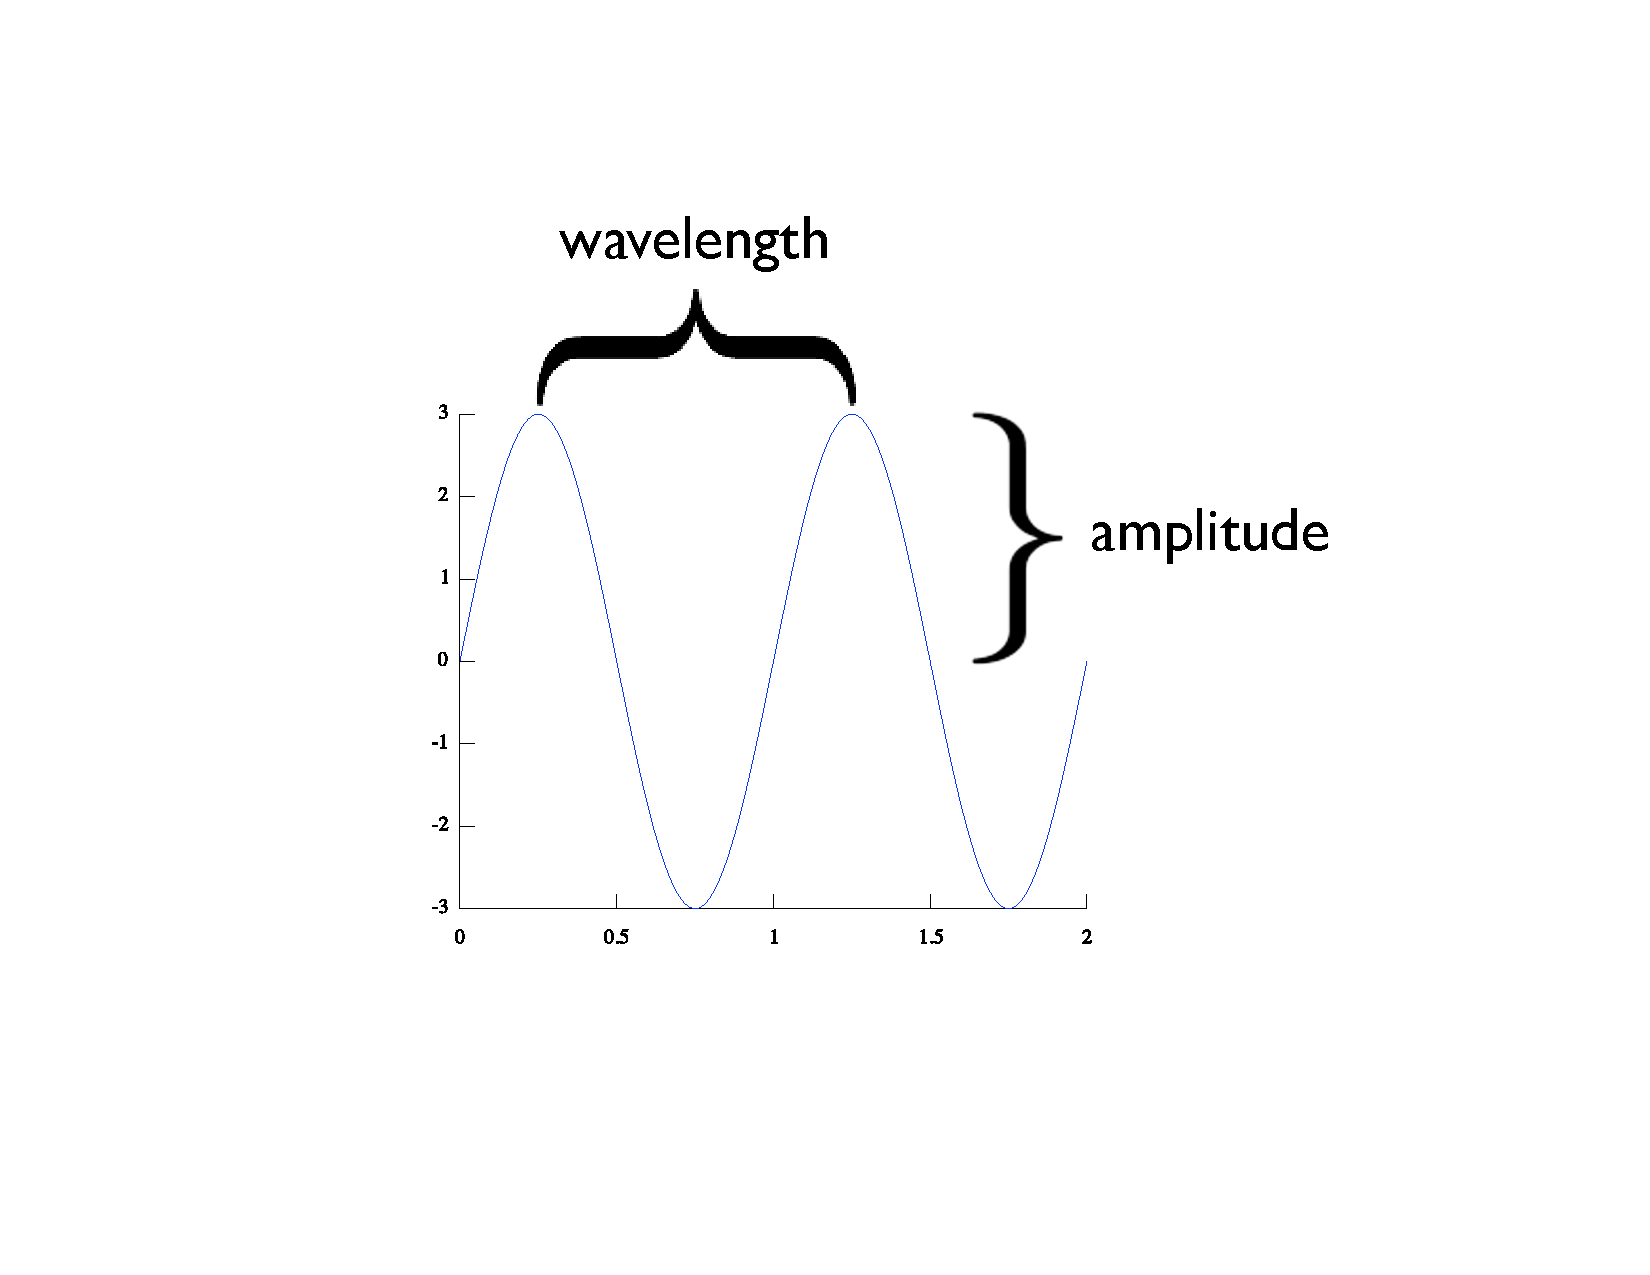
\includegraphics[scale=0.5]{charwave.pdf}
%\caption{A sin wave}
%\label{fig:gap}
%\end{center}
%\end{figure}


%\[\mathrm{amplitude}\cdot \sin ((\mathrm{frequency})\cdot t)\]

To code Figure~\ref{fig:gap} in MATLAB, use:

\begin{verbatim}
t = 0:.01:1;
amp = 3;
freq = 1;
phase = 0
y = amp*sin(freq*2*pi*t + phase);
\end{verbatim}

\subsubsection{Hearing Sine Waves}
The sine wave represents a pure tone.  To hear one, we use the MATLAB function {\tt sound()}, which converts a vector into sound.  Find the frequency that is specified, and compare to human range of hearing.  Should we be able to hear this sound?


\begin{verbatim}
freq = 1000;                
samp_rate = 1e4;
duration = 1;
samples = 0 : (1/samp_rate) : duration;
sound_wave = sin(2 * pi * samples * freq);
sound(sound_wave, samp_rate);
\end{verbatim}
{\it Enter the above code into Matlab to hear the sound.}


\subsection{Adding Sine Waves}
We can add together multiple sin waves to accomplish different shapes.  For example, if we add the wave $[4\cdot \sin(2\pi t)]$ and the wave  $[\sin(6\cdot(2\pi t))]$ we get:

%\begin{figure}[htbp]
%\begin{center}
%  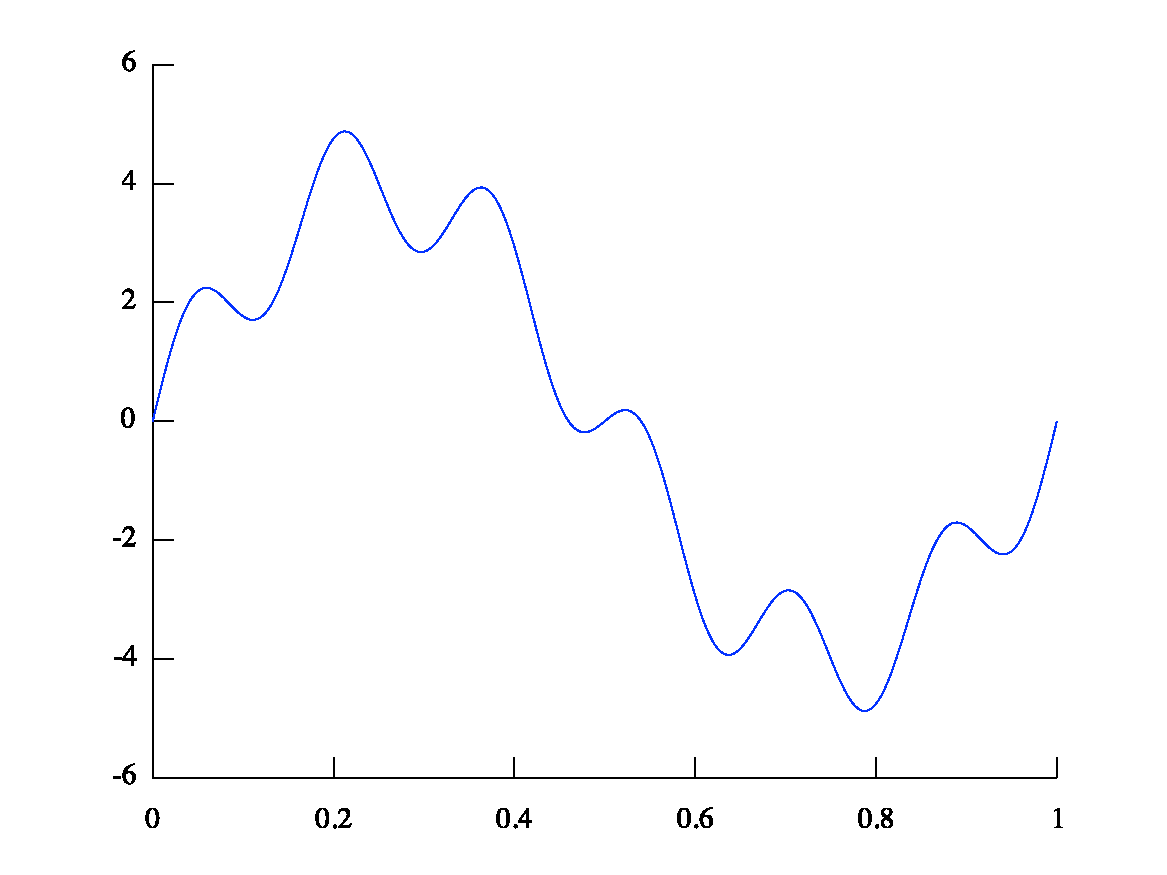
\includegraphics[scale=0.5]{compoundwv_1.pdf}
%\caption{A compound wave: $4\cdot \sin(2\pi t)+\sin(6\cdot(2\pi t))$}
%\label{default}
%\end{center}
%\end{figure}
Look at the figure and try to identify the effect of each wave.  The first wave has frequency $1$ and amplitude $4$.  This accounts for the large up-and-down motion that only goes through one cycle in the figure.  The second wave has frequency $6$ (wavelength $\frac{1}{6}$) and amplitude $1$.  This accounts for the small wiggles that happen many times in the figure.\\

Figure 4 is implemented in MATLAB with the following code:

\begin{verbatim}
t = 0:.01:1;
y = 4*sin(2*pi*t)+sin(6*2*pi*t);
plot(t,y)
\end{verbatim}
A wave of any shape can be expressed as a sum of sin and cosine waves, although it may take infinitely many.  In the end of this module we will find interesting uses for the this fact.

\subsection*{Exercises}
\paragraph{1.1} Figure \ref{fig:cwp} two shows a sum of two sine waves (with phase $0$).  Try to replicate it, and report what the amplitudes and frequencies of each wave is.

%\begin{figure}[ht]
%\begin{center}
%  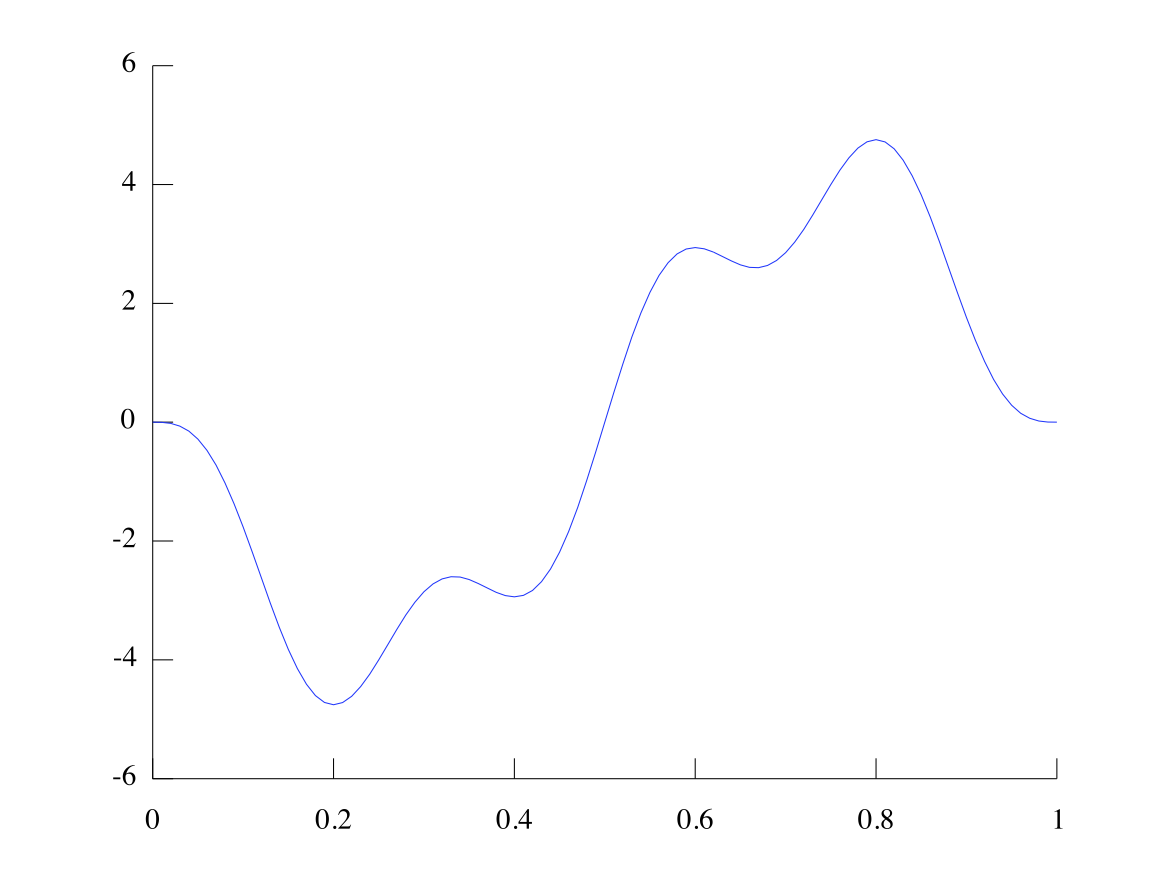
\includegraphics[scale=0.3]{comp_wave_problem.pdf}
%\label{fig:cwp}
%\caption{The compound wave for exercise 1.1}
%\end{center}
%\end{figure}


\paragraph{1.2} Use the identities $\cos(\varphi) = \sin(\varphi + \pi/2)$ and $\sin(\varphi) = \sin(\varphi+2\pi)$  to solve for $p$ in the following equations by making the above substitutions. Check your answer visually against the figures of sine and cosine waves:
%\begin{figure}[ht]
%\begin{center}
%\centerline{  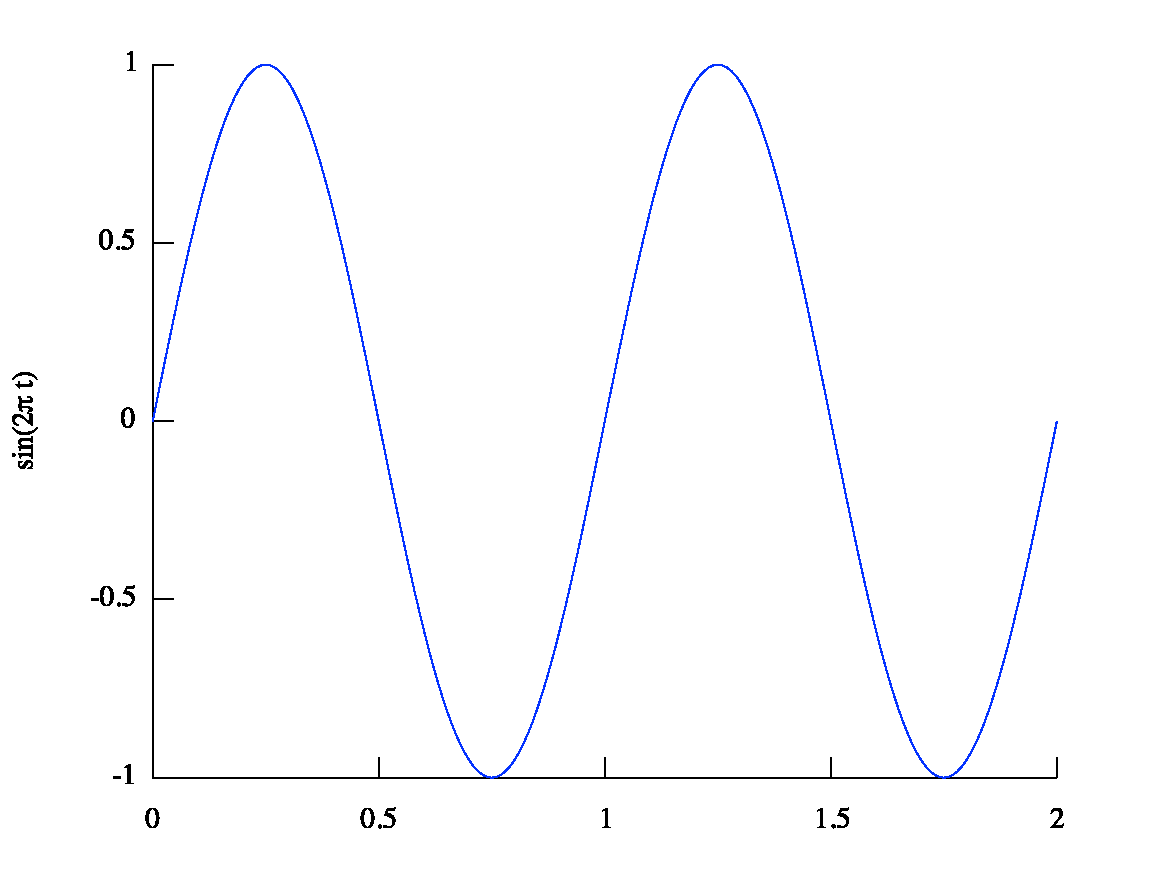
\includegraphics[scale=0.3]{sine_wv.pdf}\hspace*{.2in}
%    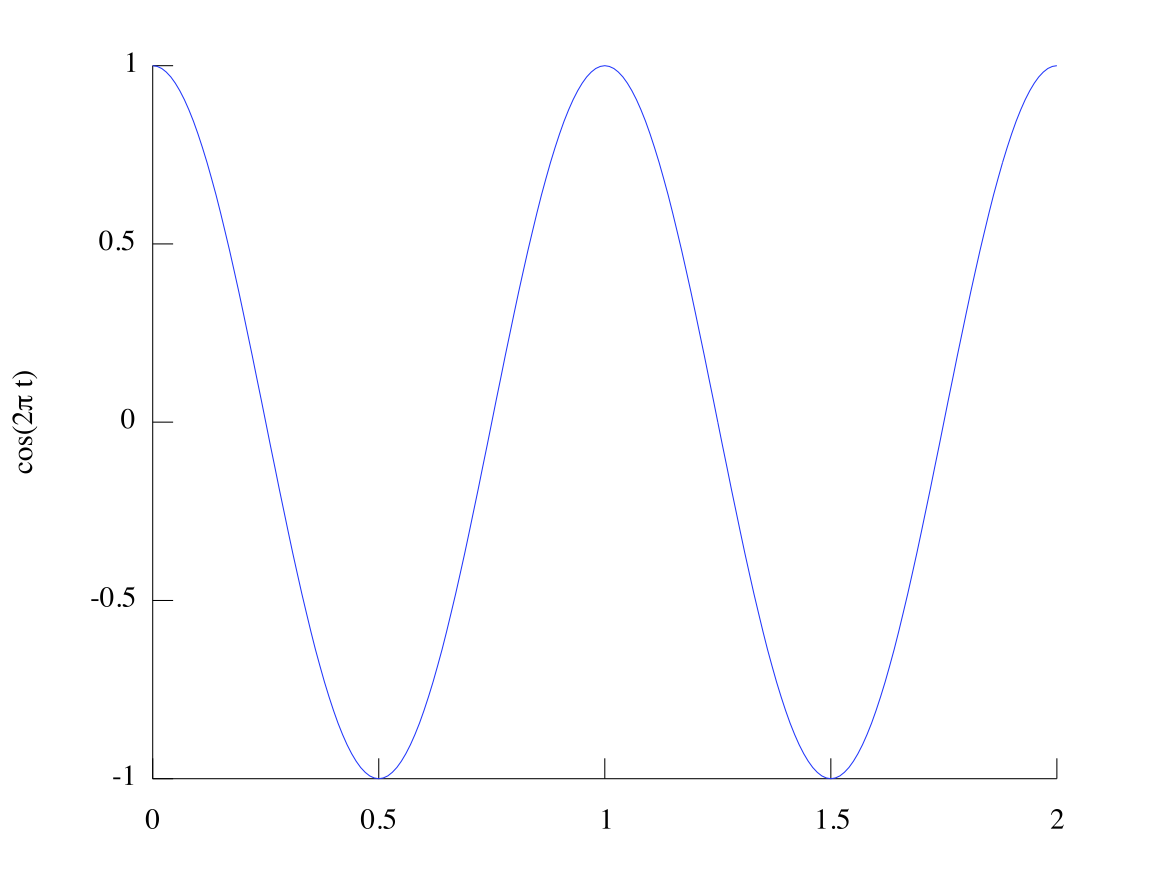
\includegraphics[scale=0.3]{cosine_wv.pdf}}
%\caption{Sine and Cosine waves.}
%\label{fig:sc}
%\end{center}
%\end{figure}

\paragraph{Equations:}
\begin{enumerate}
\item{ $\cos(\varphi + 1) = \sin(\varphi + p)$}
\item{$\sin(\varphi) = -\sin(\varphi + p) $}
\item{$\tan(\varphi)  = \frac{\sin(\varphi)}{\sin{\varphi + p}}$}
\item{$\cos(\varphi) = -\tan(\varphi + p)\cdot \cos(\varphi - p) $}
\end{enumerate}
($\tan(\varphi)$ is defined in exercise 1)

\section{Finding area under a curve (Integration)}
\subsection{Trapezoid Rule}
A useful tool for analyzing curves is finding the area underneath them.   When we have an unknown combination of waves, we can estimate the area under the curve using the {\it trapezoid rule}.  We will use $f(t)=\sin(t)$ as an example. If we were to estimate part of the area under the curve with one trapezoid, we might do the following:\\
%\begin{figure}[htbp]
%\begin{center}
%  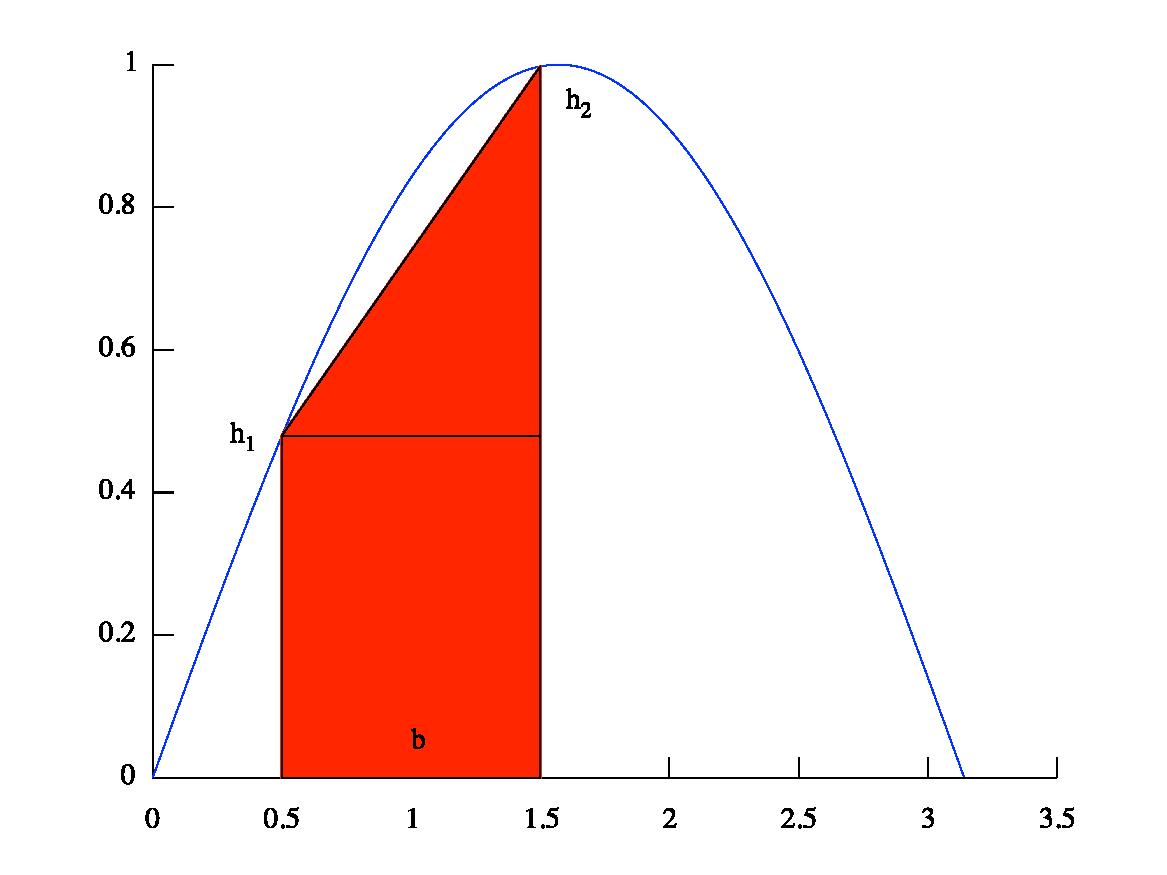
\includegraphics[scale=0.4]{first_trapezoid.pdf}
%    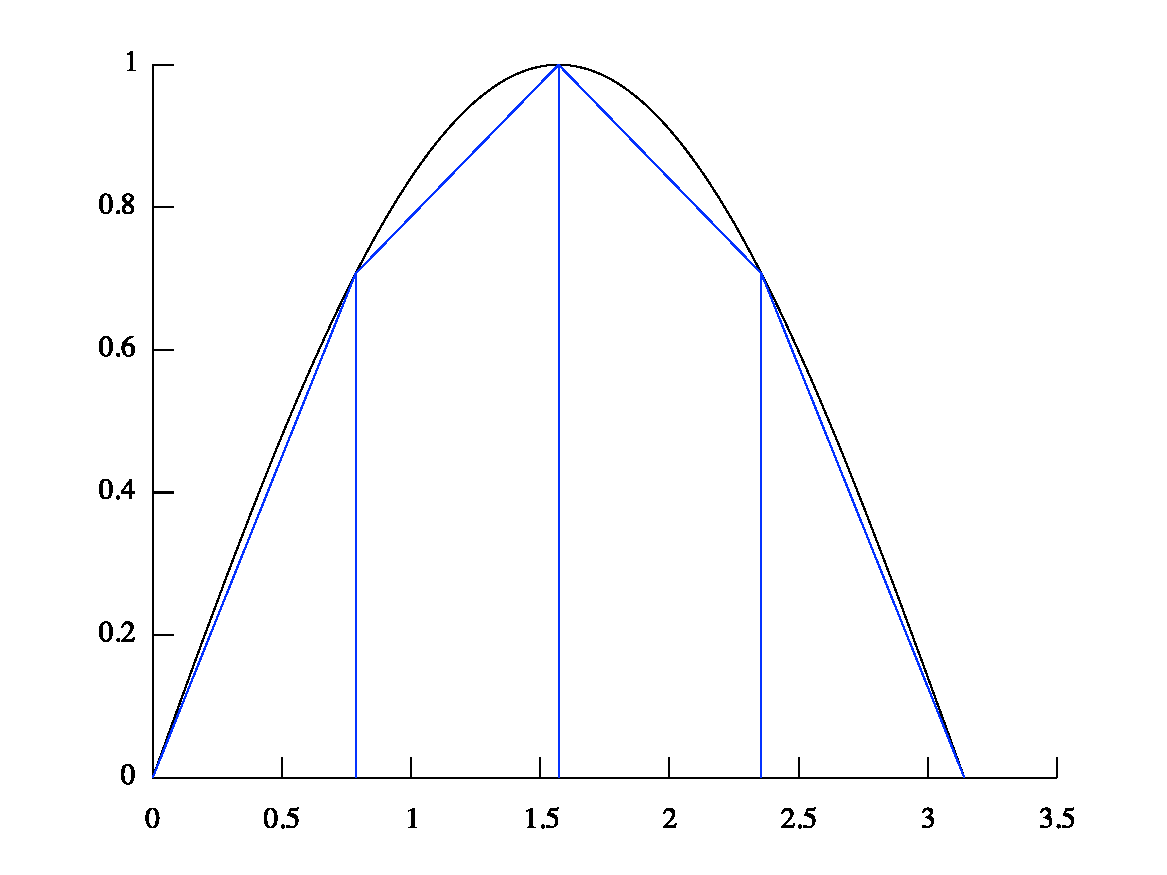
\includegraphics[scale=0.4]{fourtrap.pdf}
%\caption{Applying the trapezoid rule to a sine wave.}
%\label{default}
%\end{center}
%\end{figure}

We have labeled the two heights, $h_1$ and $h_2$, and the length of the base $b$.  The area of the square is:
\[\text{area of square} =(\text{base})\times(\text{height})=b\cdot h_1\]
The area of the top triangle is:
\[\text{area of triangle} = \frac{(\text{base})\times(\text{height})}{2}=\frac{b\cdot (h_2-h_1)}{2}\]

The total area of the trapezoid is then: 

\[\text{area of trapezoid}= b\cdot h_1 + \frac{b\cdot (h_2-h_1)}{2} = \frac{b\cdot (h_2+h_1)}{2}
\]

If we know that the two points on the $x$-axis are $t_1$ and $t_2$, then $b = t_2-t_1$.  In the figure above, $t_1 = .5$ and $t_2=1.5$.  Then the heights follow from the function: $h_1= f(t_1)=\sin(t_1)$ and $h_2= f(t_2)=\sin(t_2)$.  Thus in general, the area of a trapezoid approximating the area under $f$ between the points $t_1$ and $t_2$ is:
\begin{equation}
\label{trprule}
\text{area of trapezoid}=   \frac{b\cdot (h_2+h_1)}{2}=(t_2-t_1)\frac{f(t_1)+f(t_2)}{2}
\end{equation}


In order to get a good estimate, we split up the domain of the function $f(t)$ into several intervals $[t_i, t_{i+1}]$.  For each interval, we calculate the area of the trapezoid that approximates the area under that curve.  For example, we could approximate $f(t)$ over $[0,1]$ using four equal intervals.
%$[0,\pi/4],\ [\pi/4,\pi/2],\ [1/2, 3/4],\  [3/4,1]$.  
This would look like:\\



In this case, our estimate would be 

\[\text{approximate area of curve} = (t_2-t_1)\frac{f(t_1)+f(t_2)}{2} + \dots + (t_4-t_3)\frac{f(t_3)+f(t_4)}{2}
\]


As we take smaller and smaller intervals, our approximation will get better, because there will be less space between the trapezoids and the curve.  We can prove that the trapezoid rule given `order 2' convergence--that is, if we cut our intervals in half, our error gets four times smaller.\\
  In the general case, if we split up the domain of the function at points $\{t_1,t_2,\dots,t_n\}$, then the rule for the estimate is
\begin{equation}
\text{approximate area of curve} = (t_{1}-t_2)\frac{f(t_1)+f(t_{2})}{2}+\dots + (t_{n}-t_{n-1})\frac{f(t_{n-1})+f(t_{n})}{2}
\label{eq:area}
\end{equation}

This formula can be further reduced, which is the subject of Exercise 2.1.  

\subsection{Coding the trapezoid rule}
Here we present a code that uses the trapezoid rule to find the area under any function we provide.  We need a vector {\tt x} that holds the values of the domain, for example {\tt x = 0:.01:pi}.  We then need a vector {\tt y} that holds the function values at those {\tt x} points, for example {\tt y = sin(x)}.  

\begin{verbatim}
function curve_area = mytrapz(x, y, fast)
% function curve_area = mytrapz(x, y, fast)
%
% mytrapz.m performs the trapezoid rule on the vector given by x and y.
%
% Input:
%   x - a vector containing the domain of the function
%   y - a vector containing values of the function corresponding to the
%   values in 'x'

curve_area = 0;
    
 %loop through and add up trapezoids for as many points as we are given
for n = 2 : numel(x)
\end{verbatim}

We start the code with zero area under the curve, since we haven't counted anything yet.  Then we create a {\tt for} loop to count each triangle individually.  As we see above, more trapezoids leads to better answers, so we want to use as many trapezoids as we possibly can.  In this situation, that means using every point in {\tt x} and {\tt y}.  The function {\tt numel} simply counts the number of elements in {\tt x}.  We then calculate the area of the current triangle (within the loop):

\begin{verbatim}
    height = (y(n) + y(n-1))/2;     %average height of function across interval
    base = x(n) - x(n-1);      	    %length of interval
\end{verbatim}
The area, as in Equation (\ref{trprule}), is base times height.  The height is the average of the height of the function at the two corner points.  The length of the interval is the difference between the two corner points.

Lastly, we compute the area of the trapezoid and add it to our answer:
\begin{verbatim}
   trap_area = base * height; 	    %area of trapezoid
   curve_area = curve_area + trap_area;    %add to continuing sum
end
\end{verbatim}
The {\tt end} statement closes the loop over triangles.\\

To check the accuracy of our code, we test it with many examples, one of which is shown here.  The function {\tt trapz()} is a built-in function that performs the same operation:

\begin{verbatim}
>> x = 0:.01:pi;
>> y = sin(x);
>> mytrapz(x,y)

   ans =  1.99998206504367
   
>> trapz(x,y)

   ans =  1.99998206504367

\end{verbatim}

Additionally, we know that $\int_0^\pi \sin(x)dx=2$, so the answer we are getting is very close to the true value.

A simpler implementation of the code is included at the end, if we specify a third argument `{\tt fast}':

\begin{verbatim}
    %alternate (fast) implementation
    curve_area = sum(y(2:end-1).*(x(3:end) - x(1:end-2)));
    curve_area = curve_area + y(1)*(x(2) - x(1)) + y(end)*(x(end) - x(end-1));
    curve_area = curve_area/2;
\end{verbatim}

The explanation for this code is left as exercise 2.1.

\subsection{Integration and the Trapezoid Rule}
The trapezoid rule is a way of estimating the area under a function.  This is exactly what we call an {\it integral}.  The integral of $f(x)$ from $a$ to $b$ looks like this:
\[\int_a^b f(x) dx\]
For well-behaved functions, evaluation of the trapezoid rule approaches the true value of the integral (true area underneath the curve) as we evaluate smaller and smaller intervals.  Of course, there are other ways to characterize integration, namely the {\bf Fundamental Theorem of Calculus}.  For more on this, see the Connexions module {\it Integration, Average Behavior: The Fundamental Theorem of Calculus}.

\subsection{Exercises}
{\bf 2.1} Show that Equation \ref{eq:area} is equivalent to the ``fast" version of the code:
\[\text{approximate area of curve} =\sum_{i=2}^{n-1}f(t_1)(x_{i+1}-x_{i-1}) + f(t_1)(x_2-x_1)+ f(t_n)(x_n-x_{n-1})\]
\\
{\bf 2.2} Test the accuracy of {\tt mytrapz.m} for $y = \sin(x)$ (or some other function) as you increase the number of trapezoids.  Plot your result on a {\tt loglog()} plot: on the $x$-axis, number of trapezoids, and on the $y$-axis, error.

\section{Fourier Analysis}
We now introduce the key mathematical ideas that will allow us to break down signals into their component frequencies.

\subsection{Building the Tools}
Suppose the function $f(t)$ consists of several sine waves added together:

\[f(t) = a_1\sin(1 \cdot 2\pi t) + a_2\sin(2 \cdot 2\pi t)+\dots + a_n\sin(n \cdot 2\pi t)\]

%\begin{figure}[htbp]
%\begin{center}
%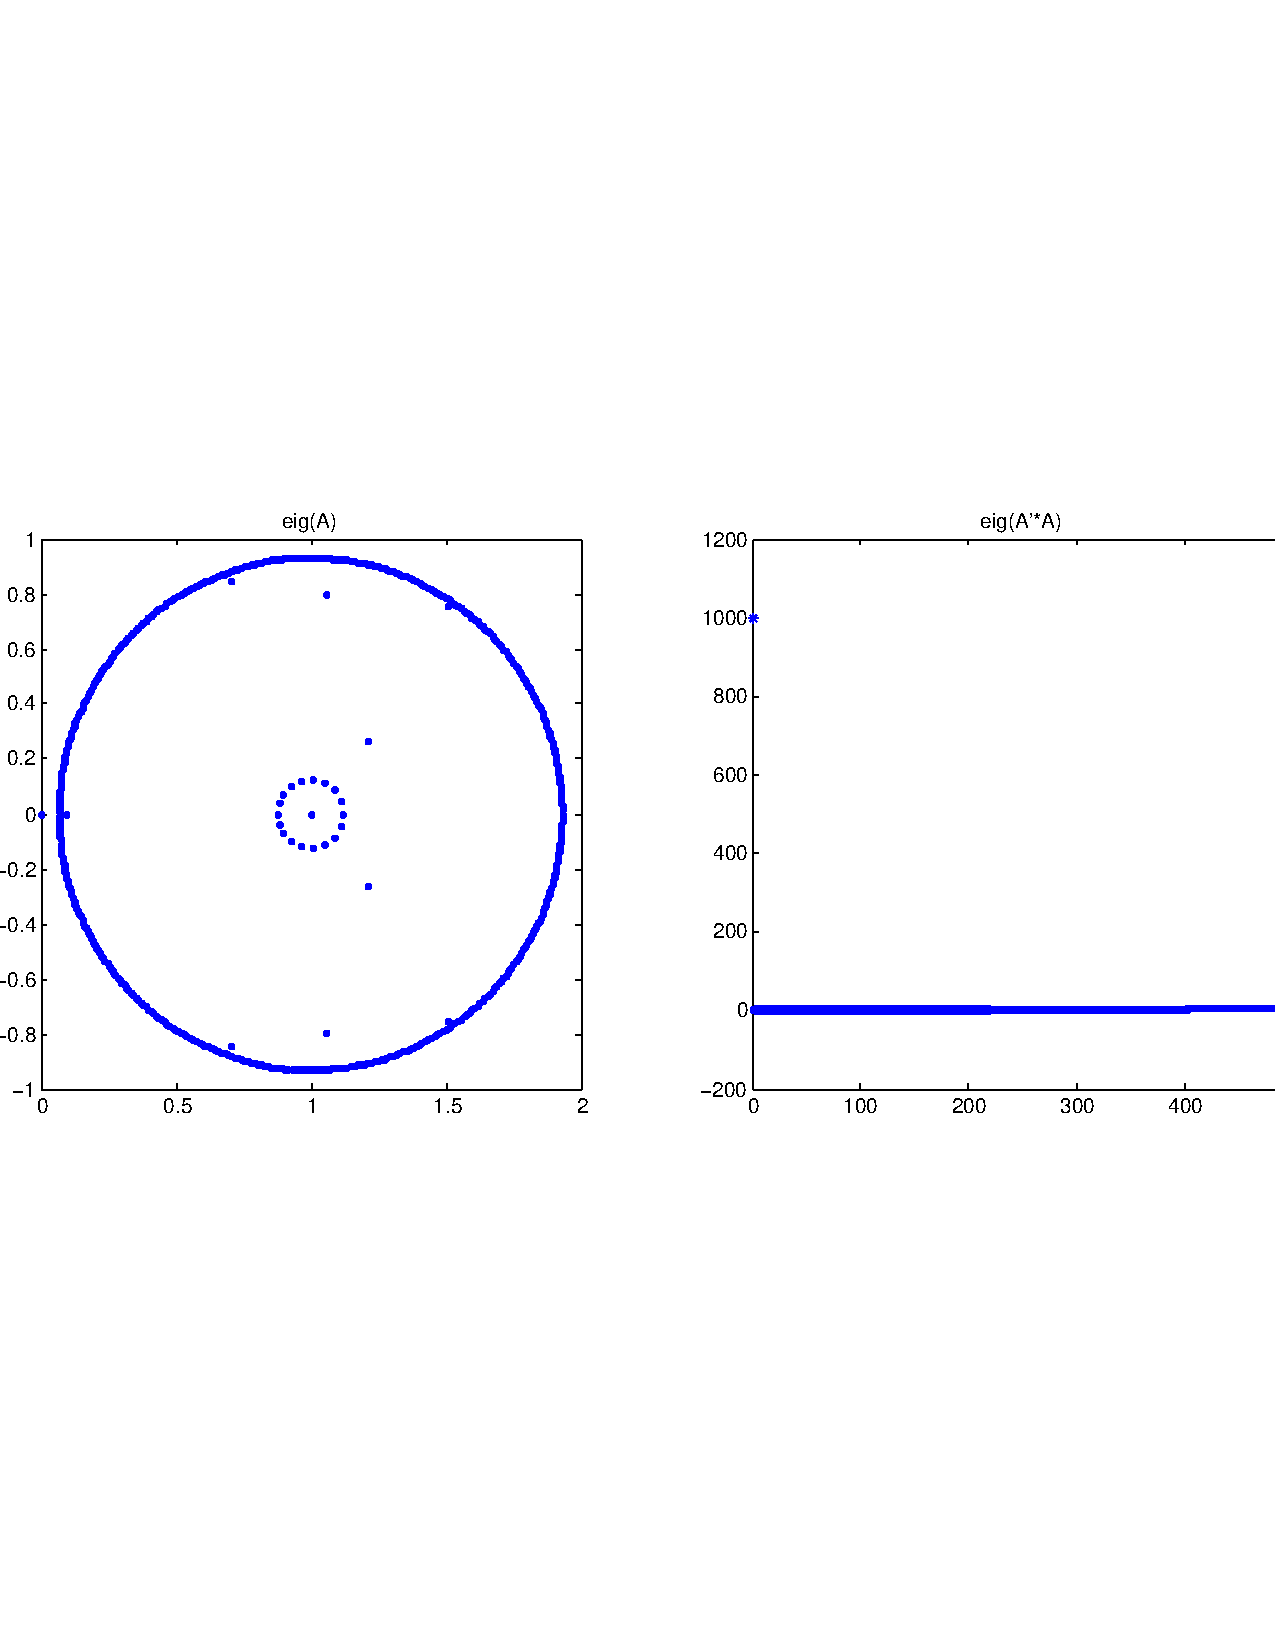
\includegraphics[clip,scale=0.5,viewport=0 0 700 600]{cmpwv2.pdf}
%\caption{A compound sine wave that we can decompose into different parts.}
%\label{default}
%\end{center}
%\end{figure}


Suppose we know $f(t)$ over some interval, say $[0,1]$, and we want to find $a_j$.  Before we jump into this, we need to calculate the value of a certain integral.   For integers $h$ and $k$, with $h\neq k$,

\begin{align*}
&\int_{0}^1 \sin(h \cdot 2\pi t)\sin(k \cdot 2\pi t) dt \\
& =  \int_{0}^1 \frac{1}{2}\left[\cos((h-k) \cdot 2\pi t) -\cos((h+k) \cdot 2\pi t) \right]dt  \qquad\qquad\qquad&\text{trigononmic identity (substitution)}\\
& =\frac{1}{2(h-k)2\pi t}\sin((h-k) \cdot 2\pi t) - \frac{1}{2(h+k)2\pi}\sin((h+k) \cdot 2\pi t)\Big|_{t=0}^1 \qquad&\text{integral of cosine is sine}\\
&  = 0&\text{evaluate from 0 to 1}
\end{align*}

If instead $h=k$,

\begin{align*}
\int_{0}^1 \sin(h \cdot 2\pi t)^2 dt & = \int_{0}^1 \frac{1}{2} (1 - \cos(2h \cdot 2\pi t))dt \qquad & \text{trigononmic identity (substitution)}\\
& = \frac{x}{2} - \frac{1}{(2h \cdot 2\pi)}\sin(2h \cdot 2\pi t)\Big |_{t=0}^1 \qquad &  \text{integral of cosine is sine}\\
& = 1/2&\text{evaluate from 0 to 1}
\end{align*}


%& = \sin(h * 2\pi t)\sin(k * 2\pi t) |_{-1}^1- \int_{0}^1 2\pi k\sin(h * 2\pi t)\cos(k * 2\pi t) dt\\
%& =-2\pi k \int_{0}^1 \sin(h * 2\pi t)\cos(k * 2\pi t) dt\\
%& = -2\pi k  \sin(h * 2\pi t)\cos(k * 2\pi t) |_{-1}^1 - (2\pi k)^2 \int_{0}^1  \sin(h * 2\pi t)\sin(k * 2\pi t) dt\\ 
%& = -4\pi k - (2\pi k)^2 \int_{0}^1  \sin(h * 2\pi t)\sin(k * 2\pi t) dt\\ 

Now we wish to find the coefficients of $f(t)$.  If we multiply $f(t)$ by $\sin(j \cdot 2\pi t)$ and integrate, we get:

\begin{align*}
& \int_{0}^{1} f(t) \sin(j \cdot 2\pi t) dt \\
 &= \int_{0}^{1} \left( a_1\sin(1 \cdot 2\pi t)\sin(j \cdot 2\pi t)+ \dots + a_j\sin(j \cdot 2\pi t)\sin(j \cdot 2\pi t)+\dots + a_n\sin(n \cdot 2\pi t)\sin(j \cdot 2\pi t)\right) dt\\
 &\qquad\qquad\qquad\qquad\qquad\qquad(\text{substitute for }f\text{ and distribute})\\
&= \int_{0}^{1}  a_1\sin(1 \cdot 2\pi t)\sin(j \cdot 2\pi t)dt+  \dots + \int_{0}^{1}  a_j\sin(j \cdot 2\pi t)\sin(j \cdot 2\pi t)dt+\dots + \int_{0}^{1}  a_n\sin(n \cdot 2\pi t)\sin(j \cdot 2\pi t)dt\\
 &\qquad\qquad\qquad\qquad\qquad\qquad(\text{the integral of a sum is the sum of integrals})\\
 & = 0 + \dots + a_j/2 + \dots + 0\\
 &\qquad\qquad\qquad\qquad\qquad\qquad(\text{all integrals are zero except for the }j^\text{th}\text{ integral by the above equations} ) \\
 & =  a_j/2
\end{align*}

Then equating the first and last lines, we have a formula for recovering $a_j$:
\begin{equation}
\label{eq:sincf}
a_j  =2 \int_0^1f(t) \sin(j \cdot 2\pi t) dt 
\end{equation}

This derivation is valid for as large of $n$ as we want.  In fact, the most general application of this is infinite series of sine waves.   \\
Additionally, we can do the same thing with sums of cosines.  If $f = b_1\cos(1 \cdot 2\pi t)+b_2\cos(2 \cdot 2\pi t)+\dots$, then we can recover the coefficients in the same way (Exercise 3.1):

\begin{equation}
\label{eq:coscf}
b_j = 2 \int_{0}^1f(t)\cos(j \cdot 2\pi t)dt
\end{equation}

And if we have a function that is a mix of the two, such as
\[f = \sin(2\pi t)+ \sin(2\cdot2\pi t) +\dots + \cos(2\pi t)+ \cos(2\cdot2\pi t) +\dots\]

we can extract the coefficients by the same equations as above (Exercise 3.2).


\subsection{Numerical Implementation}
Now we see why the trapezoid rule was so important.  In order to recover the sine coefficients of a function, we need to be able to find the integral of $f$ multiplied against different sine functions.  We can do this pretty well with our trapezoid code.  To show this method in action, we show the code {\tt myfreq.m} (full code in Appendix).  We'll walk through it here.  First, we create a sum of sine waves:

\begin{verbatim}
T = 5;			% duration of signal
dt = 0.001;     % time between signal samples
t = 0:dt:T;
N = length(t);
y = 2.5*sin(3*2*pi*t) - 4.2*sin(4*2*pi*t);    % a 2-piece wave
plot(t,y)
xlabel('time   (seconds)')
ylabel('signal')
\end{verbatim}

%\begin{figure}[htbp]
%\begin{center}
%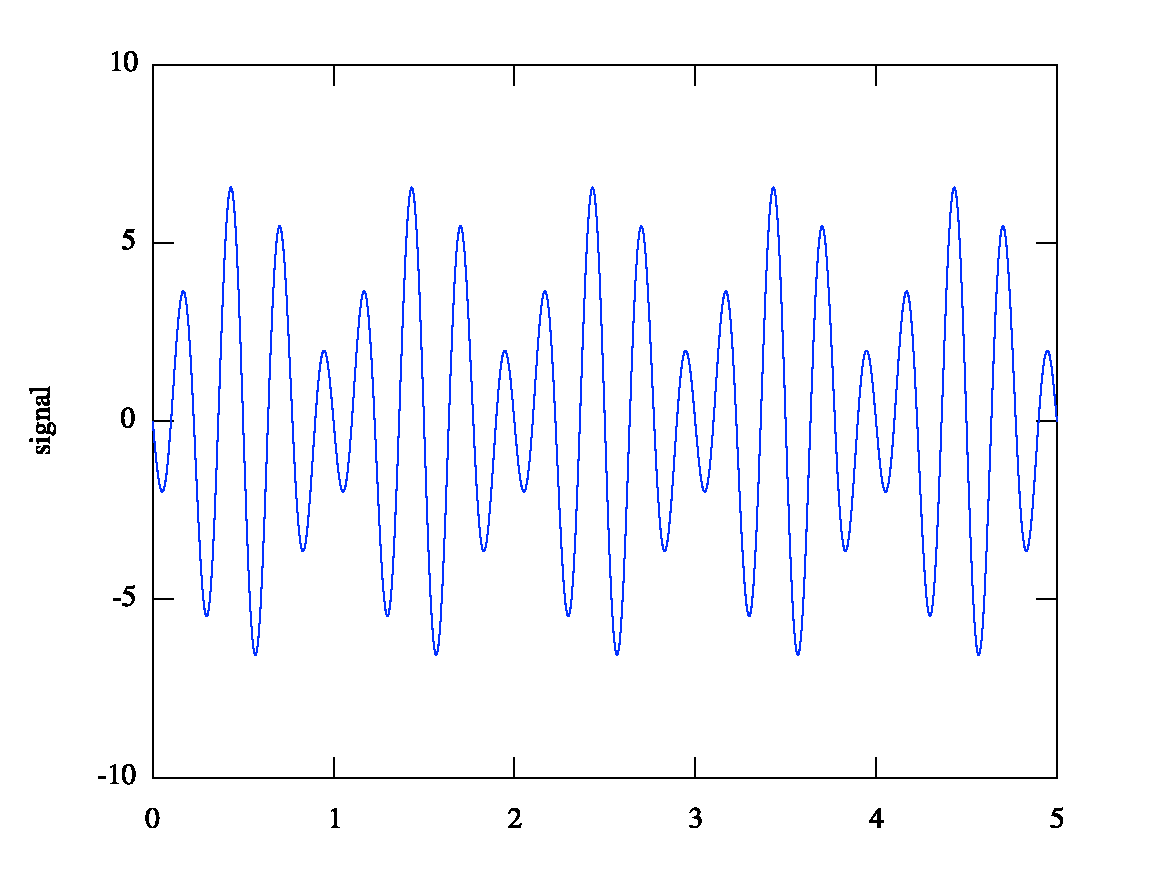
\includegraphics[scale=0.5]{mf_sine.pdf}
%\caption{The function in question}
%\label{default}
%\end{center}
%\end{figure}

Next, we use equation $(\ref{eq:sincf})$ to find the coefficients:
\begin{verbatim}
for j = 1:5,     % compute the amplitudes as ratios of areas
    a(j) = mytrapz(t,y.*sin(j*2*pi*t))/mytrapz(t,sin(j*2*pi*t).^2);
end
\end{verbatim}

Let's break down the syntax of this operation.  We loop through the computation five times, each time representing a frequency {\tt j} from $1$ to $5$.  Within the loop, the first {\tt mytrapz} is the integral we care about.  We give it two arguments: {\tt t} and {\tt y.*sin(j*2*pi*t)}.  The first, ``{\tt t}", is simply the time grid that we will approximately integrate over.  The second corresponds to $f(t)\cos(j 2\pi t)$, as in equation (\ref{eq:sincf}).  Note that {\tt j} is the frequency we are testing.  The operator ({\tt .*}) performs {\it elementwise} multiplication, that is, multiplying the corresponding elements in each array.  (Many operators such as {\tt +} and {\tt sin()} automatically do this.)  Thus each entry in the {\tt y.*sin(j*2*pi*t)} corresponds to one in {\tt t}.\\
   The second instance of {\tt mytrapz()} is just normalization (accounts for the length of the wave).  After this, we plot the recovered coefficients against the originals.  This effectively checks the error in our process.

\begin{verbatim}
figure
plot(1:5,a,'ko')    % plot the amplitudes vs frequency
hold on
plot(1:5, [0 0 2.5 -4.2 0], 'b*')
\end{verbatim}

%\begin{figure}[htbp]
%\begin{center}
%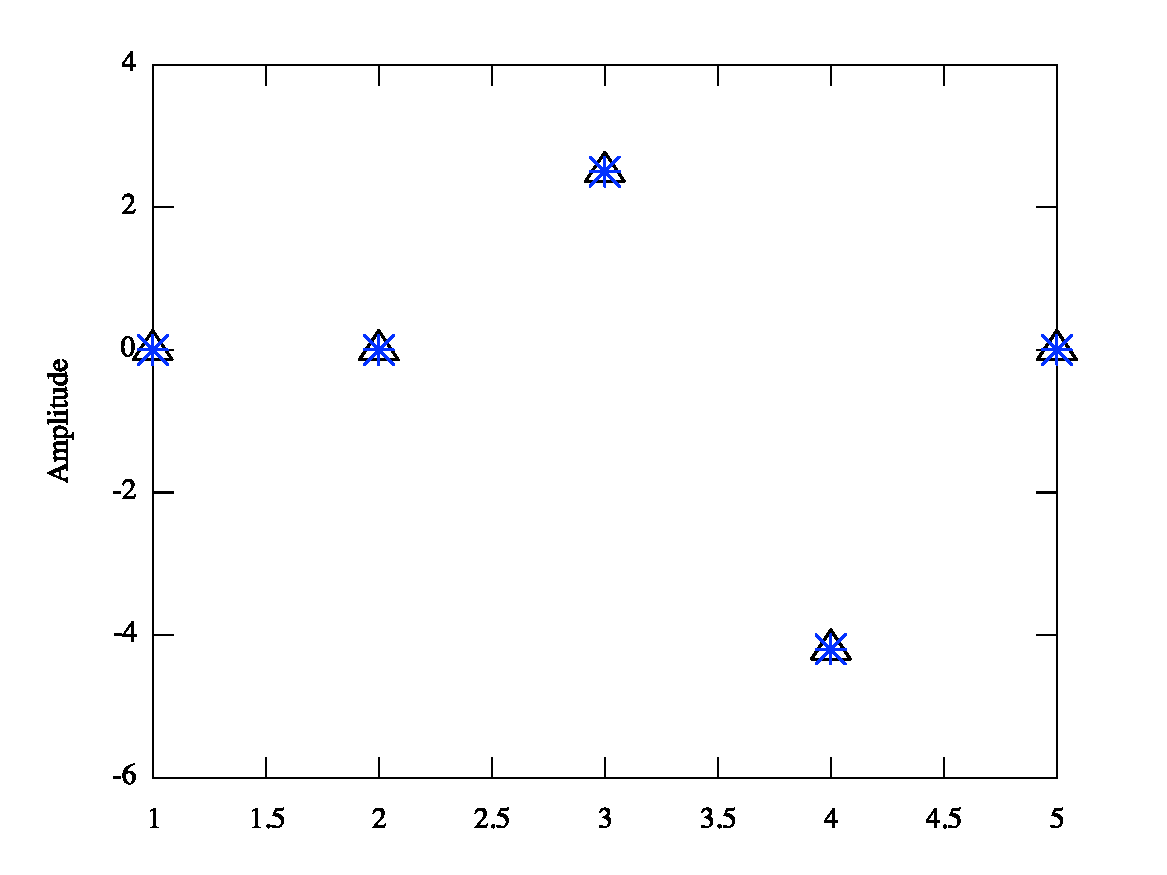
\includegraphics[scale=0.4]{checking_fourier.pdf}
%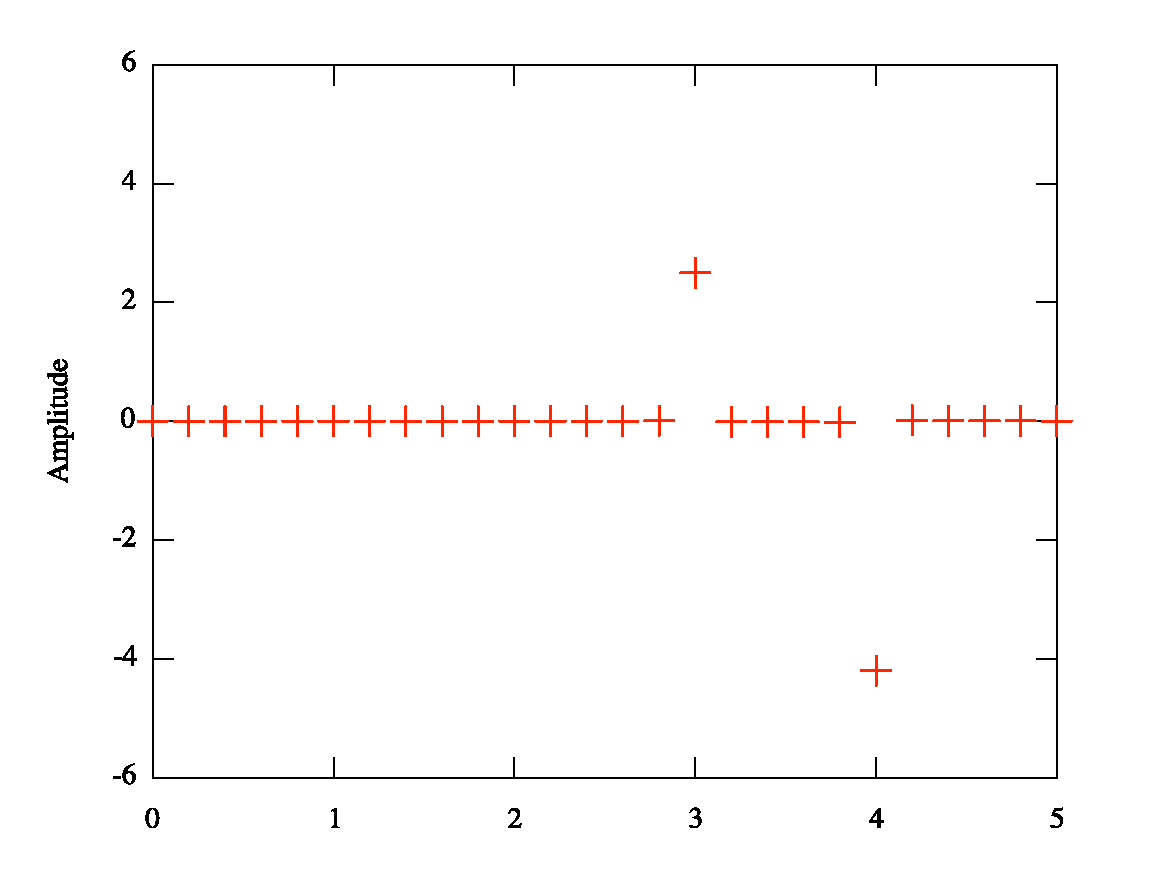
\includegraphics[scale=0.4]{mf_fft_frequencies.pdf}
%\caption{Left: Frequencies captured by {\tt myfreq()}.  Right: Frequencies captured by Matlab's {\tt fft()}}
%\label{fig:cmpmyfft}
%\end{center}
%\end{figure}

 As we can see from Figure \ref{fig:cmpmyfft}, our method works well.

The remainder of the code uses the Matlab function {\tt fft()}. This stands for ``Fast Fourier Transform."  This transforms maps a function from the {\it time} domain (the way we normally think about it) to the {\it frequency} domain.  Basically, we express a signal in terms of the frequency coefficients of which it is composed.  The plots from this analysis confirm that our analysis is the same as that of the Matlab-tested functions.


\subsection{Estimating other functions}
You may be pleasantly surprised to hear that {\it any} periodic function can be broken down into an infinite sum of sine and cosine waves.  The elements of such a sum are together called a Fourier Series.  The method for recovering the coefficients of the Fourier Series for any periodic function are the same as in equation (\ref{eq:sincf}).  Thus we create a function that will find the decomposition of any function.  We do this in {\tt myfourier.m}.  The entire code is in the appendix, but it uses very similar ideas as in {\tt myfreq()} (above).

\begin{verbatim}
function [freq mag] = myfourier(y, sr, use_fft, plot_on)
(...snip...)
freq = (0:N-1)/T;        %fft frequencies
for n = 1 : numel(freq)
    %obtain coefficient for freqency 'freq(n)'
    sinmag(n) = mytrapz(t, y.*sin(freq(n)*2*pi*t), 1);
    cosmag(n) = mytrapz(t, y.*cos(freq(n)*2*pi*t), 1);
end

\end{verbatim}

As a test, we compare the ``answer" {\tt fft} code with our own for an arbitrary function and find good agreement:

%\begin{figure}[htbp]
%\begin{center}
%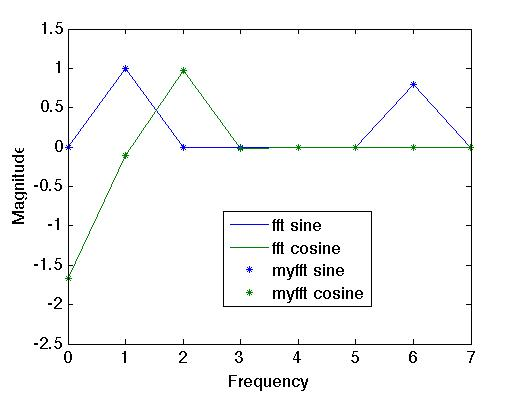
\includegraphics[scale=0.7]{myfftcoef.png}
%\caption{Comparison of {\tt myfft} to the true frequencies}
%\label{fig:fftcoef}
%\end{center}
%\end{figure}


%  To illustrate, we first try the square wave.

%\subsection{Square Wave}
%A square wave looks exactly as its sounds:

%As we add up more sine waves, we get a closer approximation to the square wave--as close as we want, in fact. 

\subsection*{Exercises}
{\bf 3.1} Suppose $f = b_1\cos(1 * 2\pi t)+b_2\cos(2 * 2\pi t)+\dots$.  Then prove Equation~\ref{eq:coscf} that helps recover the coefficients:

$$b_j = 2 \int_{0}^1f(t)\cos(j \cdot 2\pi t)dt$$
{\bf 3.2} Suppose $f$ is an infinite sum of sine and cosine waves:
\[f = \sin(2\pi t)+ \sin(2\cdot2\pi t) +\dots + \cos(2\pi t)+ \cos(2\cdot2\pi t) +\dots\]

Show that Equations (\ref{eq:sincf}) and (\ref{eq:coscf}), which give expressions for $a_j$ and $b_j$, are still valid.


\section{Applications to EEG}
Here is the application we have been seeking the whole time.  Given an EEG signal, we would like to find its corresponding Fourier series.  We have just built up the tools to decompose the signal into component frequencies.  This is useful, but the brain changes over time, and we want to be able to track changes in the signal over time.  One way to do this is the spectrogram, or the short-term Fourier transform.  It allows us to watch the way a signal changes over time.  

\subsection{Short-time Fourier Transform and Spectrogram}
The idea behind the Short-time Fourier Transform is that we break up the signal into several time windows, then take the Fourier transform of each one of these.  In Figure (\ref{fig:sgex}), we analyze the function $f(x) = \cos(4\cdot2\pi t) + 3\cos(10\cdot 2\pi t) + 5t^2 + 5\sin(35\cdot 2\pi t)$ from time $t=0$ to $t=1$.  First, we break it up into 10 segments of 100 ms each.  Each segment corresponds to one block in the ``Time" dimension.  The line in that block is the magnitudes of sine and cosine waves from the Fourier transform of the function over that time window.  The colors on the plane below it represent the magnitude of that frequency in that time interval.  The higher the magnitude, the closer to red, and the lower, the closer to blue.  The resulting image that we get is called a {\it spectrogram}.


%\begin{figure}[htbp]
%\begin{center}
%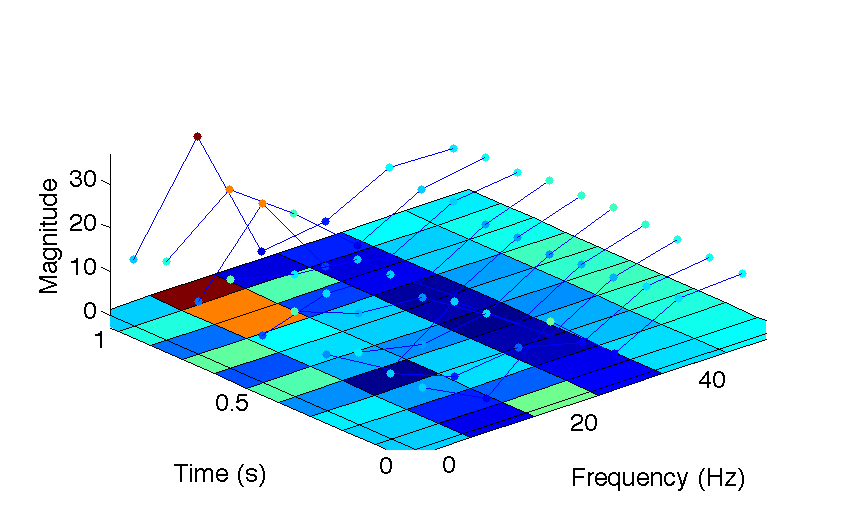
\includegraphics[scale=0.50]{sglink2}
%\caption{Visual illustration of a spectrogram}
%\label{fig:sgex}
%\end{center}
%\end{figure}

%unused:
%\begin{figure}[htbp]
%\begin{center}
%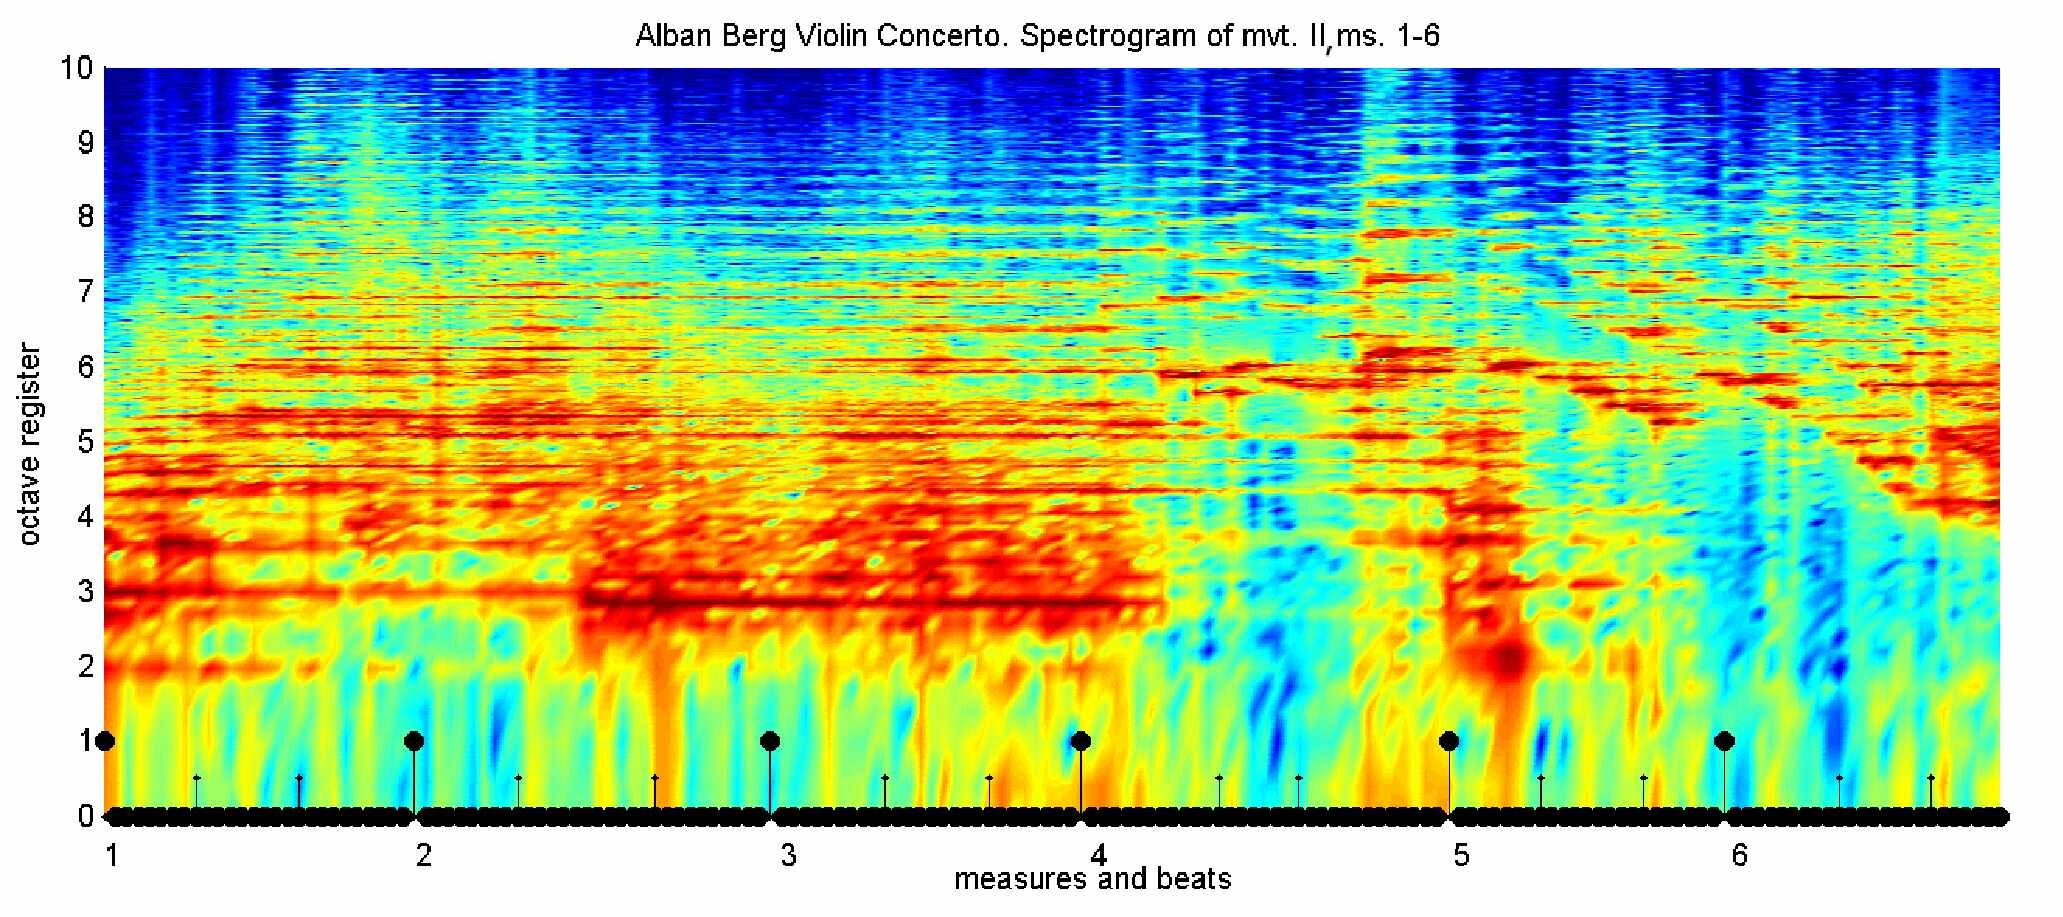
\includegraphics[scale=0.75]{sg_ex.jpg}
%\caption{The spectrogram of a violin concerto}
%\label{fig:sgex}
%\end{center}
%\end{figure}



To code something like this, we consider each time window separately.  This takes the form of a loop:

\begin{verbatim}
function [stft_plot freq tm] = my_stft(y, sr, win_len)
(...snip...)
for n = 1:Nwindow 
    %isolate the part of the signal we want to deal with
    sig_win = y((n-1)*win_len + 1 : n*win_len);
\end{verbatim}

Within this window, we perform the Fourier Transform (using our homemade code!) and record it:

\begin{verbatim}
    %perform the fourier transform
    [mg freq] = myfourier(sig_win, sr, 1);
    sm(:,n) = mg(:,1);
    cm(:,n) = mg(:,2);
end
\end{verbatim}

We then plot the results on a 2-D plane using {\tt imagesc()}.  This function associates colors with the values in the matrix, so that you can see where the values in the matrix are larger.  Thus we get a pretty picture as above.

\subsection{Testing the Spectrogram}
For the first test, we will try a simple sin wave.  

For the second test, we will use a more interesting function.  Below we have plotted $\sin(6*2\pi t)+\sin(20*2\pi t)+2*\sin(e^{t/1.5})$ over $[0,10]$.

%\begin{figure}[htbp]
%\begin{center}
%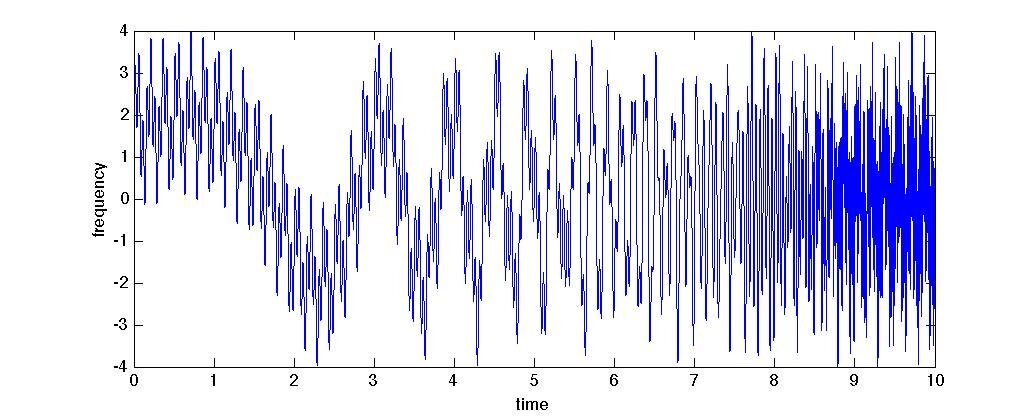
\includegraphics[scale=0.45]{sg_sig.jpg}
%\caption{An interesting signal}
%\label{default}
%\end{center}
%\end{figure}
This function is interesting because it contains a frequency component that is changing over time.  While we have waves at a constant $6$ and $20$ Hertz, the third component speeds up as $t$ gets larger and the exponential curve gets steeper.  Thus for the plot we expect to see a frequency component that is increasing.  This is exactly what we see in Figure (\ref{fig:sg})--two constant band of frequency, and one train of frequency that increases with time.

\begin{verbatim}
>> sr = 1e-4;
>> t = 0:sr:10;
>> y = sin(6*2*pi*t)+sin(20*2*pi*t)+2*sin(exp(t/1.5));
>> my_stft(y, sr, 5000);
\end{verbatim}

%\begin{figure}[htbp]
%\begin{center}
%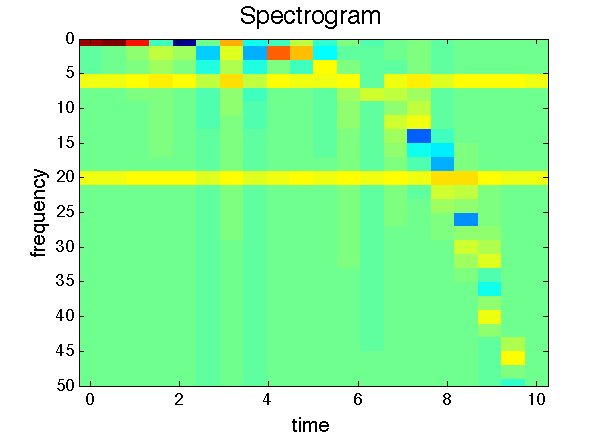
\includegraphics[scale=0.6]{sg2.png}
%\caption{The spectrogram for the above function.}
%\label{fig:sg}
%\end{center}
%\end{figure}



\subsection{Application to EEG data}
For the final section, we will analyze actual brain waves.  We recorded from and EEG, and got the signal in Figure \ref{fig:EEGwv}.
%
%\begin{figure}[htbp]
%\begin{center}
%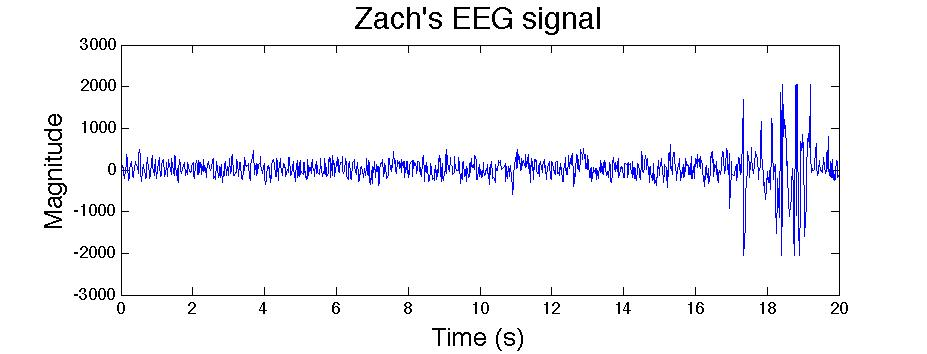
\includegraphics[scale=0.5]{EEGwv}
%\caption{An EEG wave}
%\label{fig:EEGwv}
%\end{center}
%\end{figure}

To analyze, we approximate the uneven signal as an even signal, finding the average sampling rate, in Hz.  We then call myfourier
\begin{verbatim}
octave>  avg_interval = mean(data(2:end,1)-data(1:end-1,1));
octave>  sr = 1/(avg_interval/1000);

\end{verbatim}

\section{Conclusion}
In this module we developed the tools to decompose an arbitrary signal, such as an EEG, into is component frequencies.  We began with sine waves, established the trapezoid scheme, and finally introduced Fourier analysis.  This same flavor of analysis is used in many other settings, too--see the related documents. 

\section{Code}
\subsubsection* {Code for \tt mytrapz.m}

\begin{verbatim}
function curve_area = mytrapz(x, y, fast)
% function curve_area = mytrapz(x, y, fast)
%
% mytrapz.m performs the trapezoid rule on the vector given by x and y.
%
% Input:
%   x - a vector containing the domain of the function
%   y - a vector containing values of the function corresponding to the
%   values in 'x'

if nargin < 3
    curve_area = 0;
    
    %loop through and add up trapezoids for as many points as we are given
    for n = 2 : numel(x)
        height = (y(n) + y(n-1))/2;     %average height of function across interval
        base = x(n) - x(n-1);           %length of interval
        trap_area = base * height;      %area of trapezoid
        curve_area = curve_area + trap_area;    %add to continuing sum
    end
    
elseif fast
    %alternate (fast) implementation
    curve_area = sum(y(2:end-1).*(x(3:end) - x(1:end-2)));
    curve_area = curve_area + y(1)*(x(2) - x(1)) + y(end)*(x(end) - x(end-1));
    curve_area = curve_area/2;
end
\end{verbatim}



\subsubsection* {Code for \tt myfreq.m}


\begin{verbatim}
%
% myfreq.m
%
% find the frequencies and amplitudes at which a wave is "vibrating"
%
% Contrast simple (but laborious) trapezoid computations to the fast
% and flexible built-in fft command (fft stands for fast Fourier transform).
% To make full sense of this we will need to think about complex
% numbers and the complex exponential function.
%

T = 5;			% duration of signal
dt = 0.001;     % time between signal samples
t = 0:dt:T;
N = length(t);
y = 2.5*sin(3*2*pi*t) - 4.2*sin(4*2*pi*t);    % a 2-piece wave
plot(t,y)
xlabel('time   (seconds)')
ylabel('signal')

for j = 1:5,     % compute the amplitudes as ratios of areas
    a(j) = trapz(t,y.*sin(j*2*pi*t))/trapz(t,sin(j*2*pi*t).^2);
end

figure
plot(1:5,a,'ko')    % plot the amplitudes vs frequency
hold on
plot(1:5, [0 0 2.5 -4.2 0], 'b*')


f = (0:N-1)/T;		% fft frequencies
sc = N*trapz(t,sin(2*pi*t).^2)/T;   % fft scale factor
A = fft(y);
newa = -imag(A)/sc;
plot(f,newa,'r+')


y = y + 3*cos(6*2*pi*t);    % add a cosine piece
figure(1)
hold on
plot(t,y,'g')    % plot it
hold off
legend('2 sines','2 sines and 1 cosine')

figure(2)
A = fft(y);           % take the fft of the new signal
newa = -imag(A)/sc;
plot(f,newa,'gx')
b = real(A)/sc;
plot(f,b,'gx')
xlim([0 7])   % focus in on the low frequencies
hold off
xlabel('frequency  (Hz)')
ylabel('amplitude')
legend('by hand','by fft','with cosine')
\end{verbatim}


\subsubsection*{Code for {\tt myfourier.m}}
\begin{verbatim}
% function [mag freq] = myfourier(y, dt, use_fft)
%
% myfourier.m decomposes the signal 'y', taken with sample interval dt,
% into its component frequencies.
%
% Input:
%
%   y       -- signal vection
%   dt      -- sample interval (s/sample) of y
%   use_fft -- if designated, use matlab's fft instead of trapezoid method
%
% Output:
%
%   freq -- frequency domain
%   mag  -- magnitude of frequency components of y corresponding to 'freq'

function [freq mag] = myfourier(y, dt, use_fft)

y = y(:);
N = numel(y); %number of samples
T = N*dt;                %total time
t = linspace(0,T,N)';     %reconstruct time vector
half_N = floor(N/2);  %ensures that N/2 is an integer
freq = (-half_N:half_N)'/T;   %fft frequencies

if nargin < 3  %perform explicit Fourier transform
    sinmag = zeros(size(freq));  %vector for component magnitudes
    cosmag = zeros(size(freq));  %vector for component magnitudes
    
    %loop through each frequency we will test
    for n = 1 : numel(freq)
        %obtain coefficient for freqency 'freq(n)'
        sinmag(n) = mytrapz(t, y.*sin(freq(n)*2*pi*t), 1);
        cosmag(n) = mytrapz(t, y.*cos(freq(n)*2*pi*t), 1);
    end
    
    %scale to account for sample length
    scale_factor = mytrapz(t, sin(2*pi*t).^2);
    sinmag = sinmag / scale_factor;
    cosmag = cosmag / scale_factor;
    mag = [sinmag(:)  cosmag(:)];
    
elseif use_fft   %use built-in MATLAB fft() for speed
    fft_scale_factor = mytrapz(t, sin(2*pi*t).^2) * N / T;
    A = fft(y);
    mag(:,1) = -imag(A)/fft_scale_factor;
    mag(:,2) = real(A)/fft_scale_factor;
    mag = circshift(mag, half_N);
end
\end{verbatim}


\subsubsection*{Code for {\tt mysgram.m}}
\begin{verbatim}
%
% function [stft_plot freq tm] = my_stft(y, dt, Nwindow)
%
% my_stft splits the signa 'y' into time windows, the breaks each 
% segment into its component frequencies.  See "Short-time Fourier Transform"
% 
%
% Input: 
%   y       -- signal
%   dt      -- sample interval
%   Nwindow -- number of time intervals to analyze
%
% Output:
%   stft_plot -- values plotted in the spectrogram
%   freq      -- frequency domain
%   tm        -- time domain

function [stft_plot freq tm hh] = mysgram(y, dt, Nwindow)

%count the number of windows
N = numel(y);
win_len = floor(N/Nwindow);
sm = zeros(win_len, Nwindow);
cm = zeros(win_len, Nwindow);
tm = linspace(0, numel(y) * dt, Nwindow);

%for each window
for n = 1:Nwindow 
    %isolate the part of the signal we want to deal with
    sig_win = y((n-1)*win_len + 1 : n*win_len);
    %perform the fourier transform
    [freq mg] = myfourier(sig_win, dt, 1);
    sm(:,n) = mg(1:win_len,1);
    cm(:,n) = mg(1:win_len,2);
end

stft_plot = abs(sm + cm);
stft_plot = stft_plot(round(end/2):end, :);

%plot the fourier transform over time
hh = imagesc(tm, freq(round(end/2):end), stft_plot);
title('Spectrogram', 'FontSize', 20)
xlabel('time', 'FontSize', 16)
ylabel('frequency', 'FontSize', 16)
set(gca, 'ydir', 'normal')

%just look at lower frequencies
ylim([0-win_len/2 50+win_len/2])
\end{verbatim}

\end{document}
